\documentclass[9pt,letterpaper,twoside]{article}

\usepackage[authoryear]{natbib}
\usepackage{times} 
\usepackage{amsmath,amsfonts}
\usepackage{graphicx}
\usepackage{setspace}
\usepackage{indentfirst}
\usepackage{color}
\usepackage[paper=letterpaper]{geometry}
\usepackage{fontspec}
\setmainfont[Mapping=text-tex]{Calibri}

% revise margins
\setlength{\headheight}{0.25in}
\setlength{\headsep}{-0.25in}
\setlength{\topmargin}{0.0in}
\setlength{\textheight}{9in}
\setlength{\footskip}{0.5in}
\setlength{\oddsidemargin}{0in}
\setlength{\evensidemargin}{0in}
\setlength{\textwidth}{6.5in}
\setlength{\rightskip}{0pt plus 1fil} % makes ragged right


% headings
\usepackage{fancyhdr}
\pagestyle{fancy}
\fancyfoot{}
\fancyfoot[C]{K. W. Broman}
\fancyfoot[RO, LE]{\textbf{\thepage\ SI}}
\fancyhead{}
\renewcommand{\headrulewidth}{0pt}
\renewcommand{\footrulewidth}{0pt}

\begin{document}
\thispagestyle{empty}


\vspace*{8mm}
\begin{center}

\textbf{\Large Genotype probabilities at intermediate generations\\[18pt]
in the construction of recombinant inbred lines}
 
\bigskip \bigskip
 
\bigskip \bigskip
 
\textbf{\Large SUPPLEMENT}

\bigskip \bigskip
\bigskip \bigskip
 
 
{\large Karl W. Broman\\[12pt]
Department of Biostatistics and Medical Informatics, \\[12pt]
University of Wisconsin--Madison, Madison, Wisconsin 53706 }
\end{center}


\vfill

\hfill 
{\footnotesize 14 September 2011}

\newpage

{
\centering
\includegraphics[width=\textwidth]{Figs/onelocus_fig.eps}

\bigskip
\textbf{Figure S1} {\color{white} n} One-locus genotype probabilities for 
a random individual on the autosome \textbf{(A)},  the female on the X
chromosome \textbf{(B)}, and the male on the X chromosome \textbf{(C)}, at
generation $\text{F}_k$ in the production of four-way RIL by sibling
mating, as a function of $k$.
}


\clearpage


{
\centering
\includegraphics[width=\textwidth]{Figs/riXfig.eps}

\bigskip
\textbf{Figure S2} {\color{white} n} The X chromosome in the generation of two-way (A), four-way
(B), and eight-way (C) RIL by sibling mating.
}

\clearpage

{
\centering
\includegraphics[width=\textwidth]{Figs/happrob_fig.eps}

\bigskip
\textbf{Figure S3} {\color{white} n} Two-locus haplotype probabilities, as a function of
recombination fraction, for 
a random autosome haplotype (left column),  a random X
chromosome haplotype
from the female (middle column), and the male X chromosome haplotype
(right column)  at
generation $\text{F}_k$ in the production of four-way RIL by sibling
mating, with the individual curves corresponding to different values
of $k$.
}






\newpage


\noindent \textbf{Table S1 {\color{white} n} Recursion matrix for calculating
two-locus autosomal haplotype probabilities in the generation of four-way RIL by
sibling mating}

\bigskip

{\setstretch{2.0}
{ \small \renewcommand{\arraystretch}{1.1}
\begin{center}
\begin{tabular}{cccccc} \hline
 & & &\multicolumn{3}{c}{State at $k+1$} \\
\cline{4-6}
\multicolumn{2}{c}{State at $k$} & 
& 1& 2& 3\\ \hline 
1 &
{\renewcommand{\arraystretch}{0.3}
\renewcommand{\tabcolsep}{0.5mm}
\parbox[b][3mm][c]{12mm}{
\begin{tabular}{|p{2mm}|p{2mm}||p{2mm}|p{2mm}|} \hline
$\bullet$ &           &           &           \\
$\bullet$ &           &           &           \\ \hline
\end{tabular}}}
&
& $1-r$
& $0$
& $1/4$
\\
2 &
{\renewcommand{\arraystretch}{0.3}
\renewcommand{\tabcolsep}{0.5mm}
\parbox[b][3mm][c]{12mm}{
\begin{tabular}{|p{2mm}|p{2mm}||p{2mm}|p{2mm}|} \hline
$\bullet$ &           &           &           \\
          & $\bullet$ &           &           \\ \hline
\end{tabular}}}
&
& $r$
& $0$
& $1/4$
\\
3 &
{\renewcommand{\arraystretch}{0.3}
\renewcommand{\tabcolsep}{0.5mm}
\parbox[b][3mm][c]{12mm}{
\begin{tabular}{|p{2mm}|p{2mm}||p{2mm}|p{2mm}|} \hline
$\bullet$ &           &           &           \\
          &           & $\bullet$ &           \\ \hline
\end{tabular}}}
&
& $0$
& $1$
& $1/2$
\\
\hline
\end{tabular}
\end{center} }
}

\newpage

\noindent \textbf{Table S2 {\color{white} n} Starting states for calculating
two-locus autosomal haplotype probabilities in the generation of four-way RIL by
sibling mating}

{\setstretch{2.0}
\begin{center}
\begin{tabular}{ccrlc} \hline
Prototype & No. states & \multicolumn{2}{c}{Initial pattern} & Initial probability \\ \hline
$AA$ & 4 & 
{\renewcommand{\arraystretch}{0.3}
\renewcommand{\tabcolsep}{0.5mm}
\parbox[b][3mm][c]{12mm}{
\begin{tabular}{|p{2mm}|p{2mm}||p{2mm}|p{2mm}|} \hline
$\bullet$ &           &           &           \\
$\bullet$ &           &           &           \\ \hline
\end{tabular}}}
& (1) & $1/4$ \\
$AB$ & 4 & 
{\renewcommand{\arraystretch}{0.3}
\renewcommand{\tabcolsep}{0.5mm}
\parbox[b][3mm][c]{12mm}{
\begin{tabular}{|p{2mm}|p{2mm}||p{2mm}|p{2mm}|} \hline
$\bullet$ &           &           &           \\
          & $\bullet$ &           &           \\ \hline
\end{tabular}}}
& (2) & $1/4$ \\
$AC$ & 8 & 
{\renewcommand{\arraystretch}{0.3}
\renewcommand{\tabcolsep}{0.5mm}
\parbox[b][3mm][c]{12mm}{
\begin{tabular}{|p{2mm}|p{2mm}||p{2mm}|p{2mm}|} \hline
$\bullet$ &           &           &           \\
          &           & $\bullet$ &           \\ \hline
\end{tabular}}}
& (3) & $1/8$ \\
\hline
\end{tabular}
\end{center}
}

\bigskip

\newpage

\noindent \textbf{Table S3 {\color{white} n} Transition matrix for two loci
in the generation of two-way RIL by selfing}

\bigskip

{\setstretch{1.3}
\begin{center}
{\renewcommand{\arraystretch}{1.5}\begin{tabular}{cccccc} \hline
& \multicolumn{5}{c}{$g_{k+1}$} \\ \cline{2-6}
$g_k$ & $AA|AA$ & $AB|AB$ & $AA|AB$ & $AA|BB$ & $AB|BA$  \\ \hline 
$AA|AA$ & $1$ & $0$ & $0$ & $0$ & $0$ \\ 
$AB|AB$ & $0$ & $1$ & $0$ & $0$ & $0$ \\ 
$AA|AB$ & $1/4$ & $1/4$ & $1/2$ & $0$ & $0$ \\ 
$AA|BB$ & $(1-r)^2/2$ & $r^2/2$ & $2r(1-r)$ & $(1-r)^2/2$ & $r^2/2$ \\ 
$AB|BA$ & $r^2/2$ & $(1-r)^2/2$ & $2r(1-r)$ & $r^2/2$ & $(1-r)^2/2$ \\ 
\hline
\end{tabular} }
\end{center}

}

\newpage


\noindent \textbf{Table S4 {\color{white} n} Transition matrix for one autosomal locus
in the generation of four-way RIL by sibling mating}

\bigskip

{\setstretch{1.5}
\begin{center}
\begin{tabular}{rc@{\hspace{10mm}}ccccccccccccc} \hline
 && \multicolumn{13}{c}{$g_{k+1}$} \\ \cline{3-15}
\multicolumn{2}{c}{$g_k$}  & 1 & 2 & 3 & 4 & 5 & 6 & 7 & 8 & 9 & 10 & 11 & 12 & 13\\ \hline
1: & $AA \times AA$ & 1 & 0 & 0 & 0 & 0 & 0 & 0 & 0 & 0 & 0 & 0 & 0 & 0 \\ 
2: & $AA \times AB$ & 1/4 & 1/2 & 0 & 0 & 0 & 0 & 0 & 1/4 & 0 & 0 & 0 & 0 & 0 \\ 
3: & $AA \times AC$ & 1/4 & 0 & 1/2 & 0 & 0 & 0 & 0 & 0 & 0 & 0 & 1/4 & 0 & 0 \\ 
4: & $AA \times BB$ & 0 & 0 & 0 & 0 & 0 & 0 & 0 & 1 & 0 & 0 & 0 & 0 & 0 \\ 
5: & $AA \times BC$ & 0 & 0 & 0 & 0 & 0 & 0 & 0 & 1/4 & 1/2 & 0 & 1/4 & 0 & 0 \\ 
6: & $AA \times CC$ & 0 & 0 & 0 & 0 & 0 & 0 & 0 & 0 & 0 & 0 & 1 & 0 & 0 \\ 
7: & $AA \times CD$ & 0 & 0 & 0 & 0 & 0 & 0 & 0 & 0 & 0 & 0 & 1/2 & 1/2 & 0 \\ 
8: & $AB \times AB$ & 1/8 & 1/2 & 0 & 1/8 & 0 & 0 & 0 & 1/4 & 0 & 0 & 0 & 0 & 0 \\ 
9: & $AB \times AC$ & 1/16 & 1/8 & 1/8 & 0 & 1/8 & 0 & 0 & 1/16 & 1/4 & 0 & 1/8 & 1/8 & 0 \\ 
10: & $AB \times CD$ & 0 & 0 & 0 & 0 & 0 & 0 & 0 & 0 & 0 & 0 & 1/4 & 1/2 & 1/4 \\ 
11: & $AC \times AC$ & 1/8 & 0 & 1/2 & 0 & 0 & 1/8 & 0 & 0 & 0 & 0 & 1/4 & 0 & 0 \\ 
12: & $AC \times AD$ & 1/16 & 0 & 1/4 & 0 & 0 & 0 & 1/8 & 1/16 & 1/4 & 0 & 1/8 & 1/8 & 0 \\ 
13: & $AC \times BD$ & 0 & 0 & 0 & 0 & 0 & 0 & 0 & 1/8 & 1/2 & 1/8 & 1/8 & 0 & 1/8 \\ 
\hline
\end{tabular}
\end{center}

}

\newpage


\noindent \textbf{Table S5 {\color{white} n} Probabilities for the genotypes of the 
pair of individuals at a single autosomal locus, at generation $\text{F}_{\boldsymbol{k}}$
in the formation of four-way RIL by sibling mating}

\bigskip

{\setstretch{1.7}
\begin{center} \begin{tabular}{ccc} \hline
Prototype & No. states & Probability of each \\ \hline 
$AA \times AA$ & 4 & $\frac{1}{4} + \frac{1}{4}\left(\frac{1}{2}\right)^k - \frac{1}{20}\left(\frac{1}{4}\right)^k - \left(\frac{9+4\sqrt{5}}{40}\right)\left(\frac{1+\sqrt{5}}{4}\right)^k - \left(\frac{9-4\sqrt{5}}{40}\right)\left(\frac{1-\sqrt{5}}{4}\right)^k$ \\ 
$AA \times AB$ & 4 & $\frac{1}{6}\left(-\frac{1}{4}\right)^k+\frac{1}{10}\left(\frac{1}{4}\right)^k-\frac{1}{6}\left(\frac{1}{2}\right)^k-\left(\frac{1-\sqrt{5}}{20}\right)\left(\frac{1+\sqrt{5}}{4}\right)^k - \left(\frac{1+\sqrt{5}}{20}\right)\left(\frac{1-\sqrt{5}}{4}\right)^k$ \\ 
$AA \times AC$ & 8 & $-\frac{1}{12}\left(-\frac{1}{4}\right)^k+\frac{1}{20}\left(\frac{1}{4}\right)^k-\frac{1}{6}\left(\frac{1}{2}\right)^k + \frac{1}{10}\left[\left(\frac{1+\sqrt{5}}{4}\right)^k + \left(\frac{1-\sqrt{5}}{4}\right)^k\right]$ \\ 
$AA \times BB$ & 2 & $\frac{1}{3}\left(-\frac{1}{4}\right)^k-\frac{2}{15}\left(-\frac{1}{8}\right)^k+\frac{1}{30}\left(\frac{1}{4}\right)^k-\frac{1}{30}\left(\frac{1}{2}\right)^k-\left(\frac{2-\sqrt{5}}{20}\right)\left(\frac{1+\sqrt{5}}{4}\right)^k-\left(\frac{2+\sqrt{5}}{20}\right)\left(\frac{1-\sqrt{5}}{4}\right)^k$ \\ 
$AA \times BC$ & 8 & $-\frac{1}{12}\left(-\frac{1}{4}\right)^k + \frac{2}{15}\left(-\frac{1}{8}\right)^k - \frac{1}{12}\left(\frac{1}{4}\right)^k + \frac{1}{30}\left(\frac{1}{2}\right)^k$ \\ 
$AA \times CC$ & 4 & $-\frac{1}{6}\left(-\frac{1}{4}\right)^k + \frac{1}{30}\left(-\frac{1}{8}\right)^k + \frac{1}{60}\left(\frac{1}{4}\right)^k - \frac{1}{30}\left(\frac{1}{2}\right)^k +\left(\frac{3-\sqrt{5}}{40}\right)\left(\frac{1+\sqrt{5}}{4}\right)^k+\left(\frac{3+\sqrt{5}}{40}\right)\left(\frac{1-\sqrt{5}}{4}\right)^k$ \\ 
$AA \times CD$ & 4 & $\frac{1}{6}\left(-\frac{1}{4}\right)^k - \frac{1}{5}\left(-\frac{1}{8}\right)^k + \frac{1}{30}\left(\frac{1}{2}\right)^k$ \\ 
$AB \times AB$ & 2 & $-\frac{2}{3}\left(-\frac{1}{4}\right)^k+\frac{2}{15}\left(-\frac{1}{8}\right)^k+\frac{1}{15}\left(\frac{1}{4}\right)^k-\frac{2}{15}\left(\frac{1}{2}\right)^k +\left(\frac{3-\sqrt{5}}{10}\right)\left(\frac{1+\sqrt{5}}{4}\right)^k+\left(\frac{3+\sqrt{5}}{10}\right)\left(\frac{1-\sqrt{5}}{4}\right)^k$ \\ 
$AB \times AC$ & 8 & $\frac{1}{6}\left(-\frac{1}{4}\right)^k-\frac{2}{15}\left(-\frac{1}{8}\right)^k-\frac{1}{6}\left(\frac{1}{4}\right)^k+\frac{2}{15}\left(\frac{1}{2}\right)^k$ \\ 
$AB \times CD$ & 1 & $\frac{2}{3}\left(-\frac{1}{8}\right)^k+\frac{1}{3}\left(\frac{1}{4}\right)^k$ \\ 
$AC \times AC$ & 4 & $\frac{1}{3}\left(-\frac{1}{4}\right)^k-\frac{1}{30}\left(-\frac{1}{8}\right)^k+\frac{1}{30}\left(\frac{1}{4}\right)^k-\frac{2}{15}\left(\frac{1}{2}\right)^k -\left(\frac{2-2\sqrt{5}}{20}\right)\left(\frac{1+\sqrt{5}}{4}\right)^k-\left(\frac{2+2\sqrt{5}}{20}\right)\left(\frac{1-\sqrt{5}}{4}\right)^k$ \\ 
$AC \times AD$ & 4 & $-\frac{1}{3}\left(-\frac{1}{4}\right)^k + \frac{1}{5}\left(-\frac{1}{8}\right)^k+\frac{2}{15}\left(\frac{1}{2}\right)^k$ \\ 
$AC \times BD$ & 2 & $-\frac{1}{3}\left(-\frac{1}{8}\right)^k + \frac{1}{3}\left(\frac{1}{4}\right)^k$ \\ 
\hline
\end{tabular}
\end{center}

}

\newpage


\noindent \textbf{Table S6 {\color{white} n} Transition matrix for one X chromosome
locus in the generation of four-way RIL by sibling mating}

\bigskip

{\setstretch{1.5}
\begin{center}
\begin{tabular}{rc@{\hspace{10mm}}cccccccccc} \hline
 && \multicolumn{10}{c}{$g_{k+1}$} \\ \cline{3-12}
\multicolumn{2}{c}{$g_k$}  & 1 & 2 & 3 & 4 & 5 & 6 & 7 & 8 & 9 & 10\\ \hline
1: & $AA \times A$ & 1 & 0 & 0 & 0 & 0 & 0 & 0 & 0 & 0 & 0 \\ 
2: & $AA \times B$ & 0 & 0 & 0 & 1 & 0 & 0 & 0 & 0 & 0 & 0 \\ 
3: & $AA \times C$ & 0 & 0 & 0 & 0 & 0 & 1 & 0 & 0 & 0 & 0 \\ 
4: & $AB \times A$ & 1/4 & 1/4 & 0 & 1/2 & 0 & 0 & 0 & 0 & 0 & 0 \\ 
5: & $AB \times C$ & 0 & 0 & 0 & 0 & 0 & 1/2 & 1/2 & 0 & 0 & 0 \\ 
6: & $AC \times A$ & 1/4 & 0 & 1/4 & 0 & 0 & 1/4 & 0 & 1/4 & 0 & 0 \\ 
7: & $AC \times B$ & 0 & 0 & 0 & 1/4 & 1/4 & 0 & 1/4 & 1/4 & 0 & 0 \\ 
8: & $AC \times C$ & 0 & 0 & 0 & 0 & 0 & 1/4 & 0 & 1/4 & 1/4 & 1/4 \\ 
9: & $CC \times A$ & 0 & 0 & 0 & 0 & 0 & 0 & 0 & 1 & 0 & 0 \\ 
10: & $CC \times C$ & 0 & 0 & 0 & 0 & 0 & 0 & 0 & 0 & 0 & 1 \\ 
\hline
\end{tabular}
\end{center}

}

\newpage

\noindent \textbf{Table S7 {\color{white} n} Probabilities for the genotypes of the 
pair of individuals at a single X chromosome locus, at generation $\text{F}_{\boldsymbol{k}}$
in the formation of four-way RIL by sibling mating}

\bigskip

{\setstretch{1.7}
\begin{center} \begin{tabular}{ccc} \hline
Prototype & No. states & Probability of each \\ \hline 
$AA \times A$ & 2 & $\frac{1}{3}+\frac{1}{24}\left(-\frac{1}{2}\right)^k + \frac{1}{8}\left(\frac{1}{2}\right)^k - \left(\frac{5+2\sqrt{5}}{20}\right)\left(\frac{1+\sqrt{5}}{4}\right)^k - \left(\frac{5-2\sqrt{5}}{20}\right)\left(\frac{1-\sqrt{5}}{4}\right)^k$ \\ 
$AA \times B$ & 2 & $\frac{1}{3}\left(-\frac{1}{4}\right)^k - \frac{1}{12}\left(\frac{1}{2}\right)^k - \left(\frac{5-3\sqrt{5}}{40}\right)\left(\frac{1+\sqrt{5}}{4}\right)^k - \left(\frac{5+3\sqrt{5}}{40}\right)\left(\frac{1-\sqrt{5}}{4}\right)^k$ \\ 
$AA \times C$ & 2 & $\frac{1}{8}\left(-\frac{1}{2}\right)^k-\frac{1}{24}\left(\frac{1}{2}\right)^k-\frac{1}{3}\left(-\frac{1}{4}\right)^k+\left(\frac{5-\sqrt{5}}{40}\right)\left(\frac{1+\sqrt{5}}{4}\right)^k+\left(\frac{5+\sqrt{5}}{40}\right)\left(\frac{1-\sqrt{5}}{4}\right)^k$ \\ 
$AB \times A$ & 2 & $-\frac{1}{6}\left(\frac{1}{2}\right)^k-\frac{1}{3}\left(-\frac{1}{4}\right)^k+\left(\frac{5-\sqrt{5}}{20}\right)\left(\frac{1+\sqrt{5}}{4}\right)^k+\left(\frac{5+\sqrt{5}}{20}\right)\left(\frac{1-\sqrt{5}}{4}\right)^k$ \\ 
$AB \times C$ & 1 & $\frac{1}{3}\left(\frac{1}{2}\right)^k + \frac{2}{3}\left(-\frac{1}{4}\right)^k$ \\ 
$AC \times A$ & 2 & $-\frac{1}{4}\left(-\frac{1}{2}\right)^k-\frac{1}{12}\left(\frac{1}{2}\right)^k+\frac{1}{3}\left(-\frac{1}{4}\right)^k+\frac{\sqrt{5}}{10}\left[\left(\frac{1+\sqrt{5}}{4}\right)^k-\left(\frac{1-\sqrt{5}}{4}\right)^k\right]$ \\ 
$AC \times B$ & 2 & $\frac{1}{3}\left(\frac{1}{2}\right)^k - \frac{1}{3}\left(-\frac{1}{4}\right)^k$ \\ 
$AC \times C$ & 2 & $\frac{1}{4}\left(-\frac{1}{2}\right)^k-\frac{1}{4}\left(\frac{1}{2}\right)^k+\frac{\sqrt{5}}{10}\left[\left(\frac{1+\sqrt{5}}{4}\right)^k-\left(\frac{1-\sqrt{5}}{4}\right)^k\right]$ \\ 
$CC \times A$ & 2 & $-\frac{1}{8}\left(-\frac{1}{2}\right)^k-\frac{1}{8}\left(\frac{1}{2}\right)^k+\left(\frac{5-\sqrt{5}}{40}\right)\left(\frac{1+\sqrt{5}}{4}\right)^k+\left(\frac{5+\sqrt{5}}{40}\right)\left(\frac{1-\sqrt{5}}{4}\right)^k$ \\ 
$CC \times C$ & 1 & $\frac{1}{3} - \frac{1}{12}\left(-\frac{1}{2}\right)^k + \frac{1}{4}\left(\frac{1}{2}\right)^k - \left(\frac{5+3\sqrt{5}}{20}\right)\left(\frac{1+\sqrt{5}}{4}\right)^k-\left(\frac{5-3\sqrt{5}}{20}\right)\left(\frac{1-\sqrt{5}}{4}\right)^k$ \\ 
\hline
\end{tabular}
\end{center}

}

\newpage


\noindent \textbf{Table S8 {\color{white} n} Recursion matrix for calculating
two-locus X chromosome haplotype probabilities in the generation of four-way RIL by
sibling mating}

\bigskip

{\setstretch{2.0}
{ \small \renewcommand{\arraystretch}{1.1}
\begin{center}
\begin{tabular}{ccccccc} \hline
 & & &\multicolumn{4}{c}{State at $k+1$} \\
\cline{4-7}
\multicolumn{2}{c}{State at $k$} & 
& 1& 2& 3& 4\\ \hline 
1 &
{\renewcommand{\arraystretch}{0.3}
\renewcommand{\tabcolsep}{0.5mm}
\parbox[b][3mm][c]{12mm}{
\begin{tabular}{|p{2mm}|p{2mm}||p{2mm}|} \hline
$\bullet$ &           &           \\
$\bullet$ &           &           \\ \hline
\end{tabular}}}
&
& $(1-r)/2$
& $0$
& $1-r$
& $1/4$
\\
2 &
{\renewcommand{\arraystretch}{0.3}
\renewcommand{\tabcolsep}{0.5mm}
\parbox[b][3mm][c]{12mm}{
\begin{tabular}{|p{2mm}|p{2mm}||p{2mm}|} \hline
$\bullet$ &           &           \\
          & $\bullet$ &           \\ \hline
\end{tabular}}}
&
& $r/2$
& $0$
& $r$
& $1/4$
\\
3 &
{\renewcommand{\arraystretch}{0.3}
\renewcommand{\tabcolsep}{0.5mm}
\parbox[b][3mm][c]{12mm}{
\begin{tabular}{|p{2mm}|p{2mm}||p{2mm}|} \hline
          &           & $\bullet$ \\
          &           & $\bullet$ \\ \hline
\end{tabular}}}
&
& $1/2$
& $0$
& $0$
& $0$
\\
4 &
{\renewcommand{\arraystretch}{0.3}
\renewcommand{\tabcolsep}{0.5mm}
\parbox[b][3mm][c]{12mm}{
\begin{tabular}{|p{2mm}|p{2mm}||p{2mm}|} \hline
$\bullet$ &           &           \\
          &           & $\bullet$ \\ \hline
\end{tabular}}}
&
& $0$
& $1$
& $0$
& $1/2$
\\
\hline
\end{tabular}
\end{center} }
}

\newpage

\noindent \textbf{Table S9 {\color{white} n} Starting states for calculating
two-locus X chromosome haplotype probabilities in the generation of four-way RIL by
sibling mating}

\bigskip

{\setstretch{2.0}
\begin{center}
\begin{tabular}{ccrlc} \hline
Prototype & No. states & \multicolumn{2}{c}{Initial pattern} & Initial probability \\ \hline
$AA$ & 2 & 
{\renewcommand{\arraystretch}{0.3}
\renewcommand{\tabcolsep}{0.5mm}
\parbox[b][3mm][c]{12mm}{
\begin{tabular}{|p{2mm}|p{2mm}||p{2mm}|} \hline
$\bullet$ &           &           \\
$\bullet$ &           &           \\ \hline
\end{tabular}}}
& (1) & $1/2$ \\
$AB$ & 2 & 
{\renewcommand{\arraystretch}{0.3}
\renewcommand{\tabcolsep}{0.5mm}
\parbox[b][3mm][c]{12mm}{
\begin{tabular}{|p{2mm}|p{2mm}||p{2mm}|} \hline
$\bullet$ &           &           \\
          & $\bullet$ &           \\ \hline
\end{tabular}}}
& (2) & $1/2$ \\
$AC$ & 4 & 
{\renewcommand{\arraystretch}{0.3}
\renewcommand{\tabcolsep}{0.5mm}
\parbox[b][3mm][c]{12mm}{
\begin{tabular}{|p{2mm}|p{2mm}||p{2mm}|} \hline
$\bullet$ &           &           \\
          &           & $\bullet$ \\ \hline
\end{tabular}}}
& (4) & $1/4$ \\
$CC$ & 1 & 
{\renewcommand{\arraystretch}{0.3}
\renewcommand{\tabcolsep}{0.5mm}
\parbox[b][3mm][c]{12mm}{
\begin{tabular}{|p{2mm}|p{2mm}||p{2mm}|} \hline
          &           & $\bullet$ \\
          &           & $\bullet$ \\ \hline
\end{tabular}}}
& (3) & $1$ \\
\hline
\end{tabular}
\end{center}
}

\newpage

\noindent \textbf{Table S10 {\color{white} n} Transpose of the recursion matrix for
calculating probabilities of two-locus autosomal diplotypes of the form $\boldsymbol{\boldsymbol{AA|AA}}$,
in the generation of four-way RIL by sibling mating.  Only the
non-zero entries are shown}

\bigskip

{\setstretch{2.0}
\begin{center}
\begin{tabular}{ccclllllll} \hline
\multicolumn{2}{c}{State at $k+1$} & &
\multicolumn{7}{c}{State at $k$} \\
\cline{1-2} \cline{4-10}
1 &
{\renewcommand{\arraystretch}{0.3}
\renewcommand{\tabcolsep}{0.5mm}
\parbox[b][3mm][c]{12mm}{
\begin{tabular}{|p{2mm}|p{2mm}||p{2mm}|p{2mm}|} \hline
$\bullet$ & $\bullet$ &           &           \\
$\bullet$ & $\bullet$ &           &           \\ \hline
\end{tabular}}}
&
& 2: $(1-r)^2$
& 3: $2r(1-r)$
& 4: $r^2$
& & & & \\
2 &
{\renewcommand{\arraystretch}{0.3}
\renewcommand{\tabcolsep}{0.5mm}
\parbox[b][3mm][c]{12mm}{
\begin{tabular}{|p{2mm}|p{2mm}||p{2mm}|p{2mm}|} \hline
$\bullet$ &           & $\bullet$ &           \\
$\bullet$ &           & $\bullet$ &           \\ \hline
\end{tabular}}}
&
& 1: $\frac{[r^2+(1-r)^2]}{4}$
& 2: $\frac{(1-r)^2}{2}$
& 3: $r(1-r)$
& 4: $\frac{r^2}{2}$
& 5: $\frac{(1-r)^2}{4}$
& 6: $\frac{r^2}{4}$
& 7: $r(1-r)$
\\
3 &
{\renewcommand{\arraystretch}{0.3}
\renewcommand{\tabcolsep}{0.5mm}
\parbox[b][3mm][c]{12mm}{
\begin{tabular}{|p{2mm}|p{2mm}||p{2mm}|p{2mm}|} \hline
$\bullet$ &           & $\bullet$ &           \\
$\bullet$ &           &           & $\bullet$ \\ \hline
\end{tabular}}}
&
& 8: $\frac{1-r}{2}$
& 9: $\frac{r}{2}$
& 10: $\frac{1}{2}$
& & & & \\
4 &
{\renewcommand{\arraystretch}{0.3}
\renewcommand{\tabcolsep}{0.5mm}
\parbox[b][3mm][c]{12mm}{
\begin{tabular}{|p{2mm}|p{2mm}||p{2mm}|p{2mm}|} \hline
$\bullet$ &           & $\bullet$ &           \\
          & $\bullet$ &           & $\bullet$ \\ \hline
\end{tabular}}}
&
& 2: $\frac{1}{8}$
& 3: $\frac{1}{4}$
& 4: $\frac{1}{8}$
& 11: $\frac{1}{8}$
& 12: $\frac{1}{4}$
& 13: $\frac{1}{8}$
& \\
5 &
{\renewcommand{\arraystretch}{0.3}
\renewcommand{\tabcolsep}{0.5mm}
\parbox[b][3mm][c]{12mm}{
\begin{tabular}{|p{2mm}|p{2mm}||p{2mm}|p{2mm}|} \hline
$\bullet$ &           &           &           \\
$\bullet$ &           &           &           \\ \hline
\end{tabular}}}
&
& 5: $1-r$
& 6: $r$
& & & & & \\
6 &
{\renewcommand{\arraystretch}{0.3}
\renewcommand{\tabcolsep}{0.5mm}
\parbox[b][3mm][c]{12mm}{
\begin{tabular}{|p{2mm}|p{2mm}||p{2mm}|p{2mm}|} \hline
$\bullet$ &           &           &           \\
          & $\bullet$ &           &           \\ \hline
\end{tabular}}}
&
& 11: $1$
& & & & & & \\
7 &
{\renewcommand{\arraystretch}{0.3}
\renewcommand{\tabcolsep}{0.5mm}
\parbox[b][3mm][c]{12mm}{
\begin{tabular}{|p{2mm}|p{2mm}||p{2mm}|p{2mm}|} \hline
$\bullet$ & $\bullet$ &           &           \\
$\bullet$ &           &           &           \\ \hline
\end{tabular}}}
&
& 8: $1-r$
& 9: $r$
& & & & & \\
8 &
{\renewcommand{\arraystretch}{0.3}
\renewcommand{\tabcolsep}{0.5mm}
\parbox[b][3mm][c]{12mm}{
\begin{tabular}{|p{2mm}|p{2mm}||p{2mm}|p{2mm}|} \hline
$\bullet$ &           & $\bullet$ &           \\
$\bullet$ &           &           &           \\ \hline
\end{tabular}}}
&
& 5: $\frac{1-r}{4}$
& 6: $\frac{r}{4}$
& 7: $\frac{1}{4}$
& 8: $\frac{1-r}{2}$
& 9: $\frac{r}{2}$
& & \\
9 &
{\renewcommand{\arraystretch}{0.3}
\renewcommand{\tabcolsep}{0.5mm}
\parbox[b][3mm][c]{12mm}{
\begin{tabular}{|p{2mm}|p{2mm}||p{2mm}|p{2mm}|} \hline
$\bullet$ &           & $\bullet$ &           \\
          & $\bullet$ &           &           \\ \hline
\end{tabular}}}
&
& 8: $\frac{1}{4}$
& 9: $\frac{1}{4}$
& 11: $\frac{1}{4}$
& 12: $\frac{1}{4}$
& & & \\
10 &
{\renewcommand{\arraystretch}{0.3}
\renewcommand{\tabcolsep}{0.5mm}
\parbox[b][3mm][c]{12mm}{
\begin{tabular}{|p{2mm}|p{2mm}||p{2mm}|p{2mm}|} \hline
$\bullet$ & $\bullet$ &           &           \\
$\bullet$ &           & $\bullet$ &           \\ \hline
\end{tabular}}}
&
& 2: $\frac{1-r}{4}$
& 3: $\frac{1}{4}$
& 4: $\frac{r}{4}$
& 8: $\frac{1-r}{4}$
& 9: $\frac{r}{4}$
& 10: $\frac{1}{4}$
& \\
11 &
{\renewcommand{\arraystretch}{0.3}
\renewcommand{\tabcolsep}{0.5mm}
\parbox[b][3mm][c]{12mm}{
\begin{tabular}{|p{2mm}|p{2mm}||p{2mm}|p{2mm}|} \hline
$\bullet$ &           &           &           \\
          &           & $\bullet$ &           \\ \hline
\end{tabular}}}
&
& 5: $\frac{1}{4}$
& 6: $\frac{1}{4}$
& 11: $\frac{1}{2}$
& & & & \\
12 &
{\renewcommand{\arraystretch}{0.3}
\renewcommand{\tabcolsep}{0.5mm}
\parbox[b][3mm][c]{12mm}{
\begin{tabular}{|p{2mm}|p{2mm}||p{2mm}|p{2mm}|} \hline
$\bullet$ & $\bullet$ &           &           \\
          &           & $\bullet$ &           \\ \hline
\end{tabular}}}
&
& 8: $\frac{1}{2}$
& 9: $\frac{1}{2}$
& & & & & \\
13 &
{\renewcommand{\arraystretch}{0.3}
\renewcommand{\tabcolsep}{0.5mm}
\parbox[b][3mm][c]{12mm}{
\begin{tabular}{|p{2mm}|p{2mm}||p{2mm}|p{2mm}|} \hline
$\bullet$ & $\bullet$ &           &           \\
          &           & $\bullet$ & $\bullet$ \\ \hline
\end{tabular}}}
&
& 2: $\frac{1}{4}$
& 3: $\frac{1}{2}$
& 4: $\frac{1}{4}$
& & & & \\
\hline
\end{tabular}
\end{center}
}

\newpage

\noindent \textbf{Table S11 {\color{white} n} Starting states for the calculation of
probabilities of two-locus autosomal diplotypes of the form $\boldsymbol{AA|AA}$,
in the generation of four-way RIL by sibling mating}

\bigskip

{\setstretch{2.0}
\begin{center}
\begin{tabular}{ccrlc} \hline
Prototype & No. states & \multicolumn{2}{c}{Initial pattern} & Initial probability \\ \hline
$AA|AA$ & 4 & 
{\renewcommand{\arraystretch}{0.3}
\renewcommand{\tabcolsep}{0.5mm}
\parbox[b][3mm][c]{12mm}{
\begin{tabular}{|p{2mm}|p{2mm}||p{2mm}|p{2mm}|} \hline
$\bullet$ &           &           &           \\
$\bullet$ &           &           &           \\ \hline
\end{tabular}}}
& (5) & $1/4$ \\
$AB|AB$ & 4 & 
{\renewcommand{\arraystretch}{0.3}
\renewcommand{\tabcolsep}{0.5mm}
\parbox[b][3mm][c]{12mm}{
\begin{tabular}{|p{2mm}|p{2mm}||p{2mm}|p{2mm}|} \hline
$\bullet$ &           &           &           \\
          & $\bullet$ &           &           \\ \hline
\end{tabular}}}
& (6) & $1/4$ \\
$AC|AC$ & 8 & 
{\renewcommand{\arraystretch}{0.3}
\renewcommand{\tabcolsep}{0.5mm}
\parbox[b][3mm][c]{12mm}{
\begin{tabular}{|p{2mm}|p{2mm}||p{2mm}|p{2mm}|} \hline
$\bullet$ &           &           &           \\
          &           & $\bullet$ &           \\ \hline
\end{tabular}}}
& (11) & $1/8$ \\
\hline
\end{tabular}
\end{center}
}

\newpage

\noindent \textbf{Table S12 {\color{white} n} Transpose of the recursion matrix for
calculating probabilities of two-locus autosomal diplotypes of the form $\boldsymbol{AA|AB}$,
in the generation of four-way RIL by sibling mating}

\bigskip

{\setstretch{2.0}
\begin{center}
\begin{tabular}{ccclllllll} \hline
\multicolumn{2}{c}{State at $k+1$} & &
\multicolumn{7}{c}{State at $k$} \\
\cline{1-2} \cline{4-10}
1 &
{\renewcommand{\arraystretch}{0.3}
\renewcommand{\tabcolsep}{0.5mm}
\parbox[b][3mm][c]{12mm}{
\begin{tabular}{|p{2mm}|p{2mm}||p{2mm}|p{2mm}|} \hline
$\bullet$ & $\bullet$ &           &           \\
$\bullet$ & $\circ  $ &           &           \\ \hline
\end{tabular}}}
&
& 2: $(1-r)^2$
& 3: $r(1-r)$
& 4: $r(1-r)$
& 5: $r^2$
& & & \\
2 &
{\renewcommand{\arraystretch}{0.3}
\renewcommand{\tabcolsep}{0.5mm}
\parbox[b][3mm][c]{12mm}{
\begin{tabular}{|p{2mm}|p{2mm}||p{2mm}|p{2mm}|} \hline
$\bullet$ &           & $\bullet$ &           \\
$\bullet$ &           & $\circ  $ &           \\ \hline
\end{tabular}}}
&
& 1: $\frac{r^2+(1-r)^2}{4}$
& 2: $\frac{(1-r)^2}{2}$
& 3: $\frac{r(1-r)}{2}$
& 4: $\frac{r(1-r)}{2}$
& 5: $\frac{r^2}{2}$
& 6: $\frac{r(1-r)}{4}$
& 17: $\frac{r(1-r)}{4}$
\\
3 &
{\renewcommand{\arraystretch}{0.3}
\renewcommand{\tabcolsep}{0.5mm}
\parbox[b][3mm][c]{12mm}{
\begin{tabular}{|p{2mm}|p{2mm}||p{2mm}|p{2mm}|} \hline
$\bullet$ &           & $\bullet$ &           \\
$\bullet$ &           &           & $\circ  $ \\ \hline
\end{tabular}}}
&
& 7: $\frac{1}{4}$
& 8: $\frac{1-r}{4}$
& 9: $\frac{1-r}{4}$
& 10: $\frac{r}{4}$
& 16: $\frac{r}{4}$
& & \\
4 &
{\renewcommand{\arraystretch}{0.3}
\renewcommand{\tabcolsep}{0.5mm}
\parbox[b][3mm][c]{12mm}{
\begin{tabular}{|p{2mm}|p{2mm}||p{2mm}|p{2mm}|} \hline
$\bullet$ &           & $\bullet$ &           \\
          & $\bullet$ & $\circ  $ &           \\ \hline
\end{tabular}}}
&
& 9: $\frac{r}{4}$
& 10: $\frac{1-r}{4}$
& 11: $\frac{1}{4}$
& 12: $\frac{1-r}{4}$
& 13: $\frac{r}{4}$
& & \\
5 &
{\renewcommand{\arraystretch}{0.3}
\renewcommand{\tabcolsep}{0.5mm}
\parbox[b][3mm][c]{12mm}{
\begin{tabular}{|p{2mm}|p{2mm}||p{2mm}|p{2mm}|} \hline
$\bullet$ &           & $\bullet$ &           \\
          & $\bullet$ &           & $\circ  $ \\ \hline
\end{tabular}}}
&
& 2: $\frac{1}{8}$
& 3: $\frac{1}{8}$
& 4: $\frac{1}{8}$
& 5: $\frac{1}{8}$
& 14: $\frac{1}{8}$
& 15: $\frac{1}{8}$
& \\
6 &
{\renewcommand{\arraystretch}{0.3}
\renewcommand{\tabcolsep}{0.5mm}
\parbox[b][3mm][c]{12mm}{
\begin{tabular}{|p{2mm}|p{2mm}||p{2mm}|p{2mm}|} \hline
$\bullet$ &           &           &           \\
$\bullet$ & $\circ  $ &           &           \\ \hline
\end{tabular}}}
&
& 8: $(1-r)$
& 16: $r$
& & & & & \\
7 &
{\renewcommand{\arraystretch}{0.3}
\renewcommand{\tabcolsep}{0.5mm}
\parbox[b][3mm][c]{12mm}{
\begin{tabular}{|p{2mm}|p{2mm}||p{2mm}|p{2mm}|} \hline
$\bullet$ & $\bullet$ &           &           \\
$\bullet$ &           & $\circ  $ &           \\ \hline
\end{tabular}}}
&
& 2: $\frac{1-r}{4}$
& 3: $\frac{1-r}{4}$
& 4: $\frac{r}{4}$
& 5: $\frac{r}{4}$
& 9: $\frac{1-r}{4}$
& 10: $\frac{r}{4}$
& \\
8 &
{\renewcommand{\arraystretch}{0.3}
\renewcommand{\tabcolsep}{0.5mm}
\parbox[b][3mm][c]{12mm}{
\begin{tabular}{|p{2mm}|p{2mm}||p{2mm}|p{2mm}|} \hline
$\bullet$ &           &           &           \\
$\bullet$ &           & $\circ  $ &           \\ \hline
\end{tabular}}}
&
& 6: $\frac{1-r}{4}$
& 8: $\frac{1-r}{2}$
& 16: $\frac{r}{2}$
& 17: $\frac{r}{4}$
& & & \\
9 &
{\renewcommand{\arraystretch}{0.3}
\renewcommand{\tabcolsep}{0.5mm}
\parbox[b][3mm][c]{12mm}{
\begin{tabular}{|p{2mm}|p{2mm}||p{2mm}|p{2mm}|} \hline
$\bullet$ &           & $\bullet$ &           \\
$\bullet$ & $\circ  $ &           &           \\ \hline
\end{tabular}}}
&
& 2: $\frac{1-r}{4}$
& 3: $\frac{1-r}{4}$
& 4: $\frac{r}{4}$
& 5: $\frac{r}{4}$
& 7: $\frac{1}{4}$
& 8: $\frac{1-r}{4}$
& 16: $\frac{r}{4}$
\\
10 &
{\renewcommand{\arraystretch}{0.3}
\renewcommand{\tabcolsep}{0.5mm}
\parbox[b][3mm][c]{12mm}{
\begin{tabular}{|p{2mm}|p{2mm}||p{2mm}|p{2mm}|} \hline
$\bullet$ &           & $\bullet$ &           \\
$\circ  $ & $\bullet$ &           &           \\ \hline
\end{tabular}}}
&
& 2: $\frac{1-r}{4}$
& 3: $\frac{r}{4}$
& 4: $\frac{1-r}{4}$
& 5: $\frac{r}{4}$
& 11: $\frac{1}{4}$
& 12: $\frac{1-r}{4}$
& 13: $\frac{r}{4}$
\\
11 &
{\renewcommand{\arraystretch}{0.3}
\renewcommand{\tabcolsep}{0.5mm}
\parbox[b][3mm][c]{12mm}{
\begin{tabular}{|p{2mm}|p{2mm}||p{2mm}|p{2mm}|} \hline
$\bullet$ & $\bullet$ &           &           \\
$\circ  $ &           & $\bullet$ &           \\ \hline
\end{tabular}}}
&
& 2: $\frac{1-r}{4}$
& 3: $\frac{r}{4}$
& 4: $\frac{1-r}{4}$
& 5: $\frac{r}{4}$
& 9: $\frac{r}{4}$
& 10: $\frac{1-r}{4}$
& \\
12 &
{\renewcommand{\arraystretch}{0.3}
\renewcommand{\tabcolsep}{0.5mm}
\parbox[b][3mm][c]{12mm}{
\begin{tabular}{|p{2mm}|p{2mm}||p{2mm}|p{2mm}|} \hline
$\bullet$ &           &           &           \\
$\circ  $ &           & $\bullet$ &           \\ \hline
\end{tabular}}}
&
& 6: $\frac{r}{4}$
& 12: $\frac{1-r}{2}$
& 13: $\frac{r}{2}$
& 17: $\frac{1-r}{4}$
& & & \\
13 &
{\renewcommand{\arraystretch}{0.3}
\renewcommand{\tabcolsep}{0.5mm}
\parbox[b][3mm][c]{12mm}{
\begin{tabular}{|p{2mm}|p{2mm}||p{2mm}|p{2mm}|} \hline
$\bullet$ &           &           &           \\
          & $\circ  $ & $\bullet$ &           \\ \hline
\end{tabular}}}
&
& 8: $\frac{1}{4}$
& 15: $\frac{1}{4}$
& 16: $\frac{1}{4}$
& & & & \\
14 &
{\renewcommand{\arraystretch}{0.3}
\renewcommand{\tabcolsep}{0.5mm}
\parbox[b][3mm][c]{12mm}{
\begin{tabular}{|p{2mm}|p{2mm}||p{2mm}|p{2mm}|} \hline
$\bullet$ & $\bullet$ &           &           \\
          &           & $\bullet$ & $\circ  $ \\ \hline
\end{tabular}}}
&
& 2: $\frac{1}{4}$
& 3: $\frac{1}{4}$
& 4: $\frac{1}{4}$
& 5: $\frac{1}{4}$
& & & \\
15 &
{\renewcommand{\arraystretch}{0.3}
\renewcommand{\tabcolsep}{0.5mm}
\parbox[b][3mm][c]{12mm}{
\begin{tabular}{|p{2mm}|p{2mm}||p{2mm}|p{2mm}|} \hline
$\bullet$ &           &           &           \\
          &           & $\bullet$ & $\circ  $ \\ \hline
\end{tabular}}}
&
& 8: $\frac{1}{4}$
& 12: $\frac{1}{4}$
& 13: $\frac{1}{4}$
& 16: $\frac{1}{4}$
& & & \\
16 &
{\renewcommand{\arraystretch}{0.3}
\renewcommand{\tabcolsep}{0.5mm}
\parbox[b][3mm][c]{12mm}{
\begin{tabular}{|p{2mm}|p{2mm}||p{2mm}|p{2mm}|} \hline
$\bullet$ &           &           &           \\
          & $\bullet$ & $\circ  $ &           \\ \hline
\end{tabular}}}
&
& 12: $\frac{1}{4}$
& 13: $\frac{1}{4}$
& 15: $\frac{1}{4}$
& & & & \\
17 &
{\renewcommand{\arraystretch}{0.3}
\renewcommand{\tabcolsep}{0.5mm}
\parbox[b][3mm][c]{12mm}{
\begin{tabular}{|p{2mm}|p{2mm}||p{2mm}|p{2mm}|} \hline
$\bullet$ &           &           &           \\
$\circ  $ & $\bullet$ &           &           \\ \hline
\end{tabular}}}
&
& 12: $(1-r)$
& 13: $r$
& & & & & \\
\hline
\end{tabular}
\end{center}
}

\newpage

\noindent \textbf{Table S13 {\color{white} n} Starting states for the calculation of
probabilities of two-locus autosomal diplotypes of the form $\boldsymbol{AA|AB}$,
in the generation of four-way RIL by sibling mating}

\bigskip

{\setstretch{2.0}
\begin{center}
\begin{tabular}{ccrlc} \hline
Prototype & No. states & \multicolumn{2}{c}{Initial pattern} & Initial probability \\ \hline
$AA|AB$ & 8 & 
{\renewcommand{\arraystretch}{0.3}
\renewcommand{\tabcolsep}{0.5mm}
\parbox[b][3mm][c]{12mm}{
\begin{tabular}{|p{2mm}|p{2mm}||p{2mm}|p{2mm}|} \hline
$\bullet$ &           &           &           \\
$\bullet$ & $\circ  $ &           &           \\ \hline
\end{tabular}}}
& (6) & $1/2$ \\
$AA|AC$ & 16 & 
{\renewcommand{\arraystretch}{0.3}
\renewcommand{\tabcolsep}{0.5mm}
\parbox[b][3mm][c]{12mm}{
\begin{tabular}{|p{2mm}|p{2mm}||p{2mm}|p{2mm}|} \hline
$\bullet$ &           &           &           \\
$\bullet$ &           & $\circ  $ &           \\ \hline
\end{tabular}}}
& (8) & $1/4$ \\
$AB|AC$ & 16 & 
{\renewcommand{\arraystretch}{0.3}
\renewcommand{\tabcolsep}{0.5mm}
\parbox[b][3mm][c]{12mm}{
\begin{tabular}{|p{2mm}|p{2mm}||p{2mm}|p{2mm}|} \hline
$\bullet$ &           &           &           \\
          & $\bullet$ & $\circ  $ &           \\ \hline
\end{tabular}}}
& (16) & $1/4$ \\
$AC|AD$ & 8 & 
{\renewcommand{\arraystretch}{0.3}
\renewcommand{\tabcolsep}{0.5mm}
\parbox[b][3mm][c]{12mm}{
\begin{tabular}{|p{2mm}|p{2mm}||p{2mm}|p{2mm}|} \hline
$\bullet$ &           &           &           \\
          &           & $\bullet$ & $\circ  $ \\ \hline
\end{tabular}}}
& (15) & $1/4$ \\
\hline
\end{tabular}
\end{center}
}

\newpage

\noindent \textbf{Table S14 {\color{white} n} Transpose of the recursion matrix for
calculating probabilities of two-locus autosomal diplotypes of the form $\boldsymbol{AA|BB}$,
in the generation of four-way RIL by sibling mating}

\bigskip

{\setstretch{2.0}
\begin{center}
\begin{tabular}{ccclllllll} \hline
\multicolumn{2}{c}{State at $k+1$} & &
\multicolumn{7}{c}{State at $k$} \\
\cline{1-2} \cline{4-10}
1 &
{\renewcommand{\arraystretch}{0.3}
\renewcommand{\tabcolsep}{0.5mm}
\parbox[b][3mm][c]{12mm}{
\begin{tabular}{|p{2mm}|p{2mm}||p{2mm}|p{2mm}|} \hline
$\bullet$ & $\circ  $ &           &           \\
$\bullet$ & $\circ  $ &           &           \\ \hline
\end{tabular}}}
&
& 2: $\frac{(1-r)^2}{2}$
& 3: $\frac{r(1-r)}{2}$
& 4: $\frac{r(1-r)}{2}$
& 5: $\frac{r^2}{2}$
& & & \\
2 &
{\renewcommand{\arraystretch}{0.3}
\renewcommand{\tabcolsep}{0.5mm}
\parbox[b][3mm][c]{12mm}{
\begin{tabular}{|p{2mm}|p{2mm}||p{2mm}|p{2mm}|} \hline
$\bullet$ &           & $\circ  $ &           \\
$\bullet$ &           & $\circ  $ &           \\ \hline
\end{tabular}}}
&
& 1: $\frac{(1-r)^2}{2}$
& 2: $\frac{(1-r)^2}{2}$
& 3: $\frac{r(1-r)}{2}$
& 4: $\frac{r(1-r)}{2}$
& 5: $\frac{r^2}{2}$
& 6: $\frac{r^2}{2}$
& \\
3 &
{\renewcommand{\arraystretch}{0.3}
\renewcommand{\tabcolsep}{0.5mm}
\parbox[b][3mm][c]{12mm}{
\begin{tabular}{|p{2mm}|p{2mm}||p{2mm}|p{2mm}|} \hline
$\bullet$ &           & $\circ  $ &           \\
$\bullet$ &           &           & $\circ  $ \\ \hline
\end{tabular}}}
&
& 7: $\frac{1-r}{4}$
& 8: $\frac{r}{4}$
& & & & & \\
4 &
{\renewcommand{\arraystretch}{0.3}
\renewcommand{\tabcolsep}{0.5mm}
\parbox[b][3mm][c]{12mm}{
\begin{tabular}{|p{2mm}|p{2mm}||p{2mm}|p{2mm}|} \hline
$\bullet$ &           & $\circ  $ &           \\
          & $\bullet$ & $\circ  $ &           \\ \hline
\end{tabular}}}
&
& 9: $\frac{1-r}{4}$
& 10: $\frac{r}{4}$
& & & & & \\
5 &
{\renewcommand{\arraystretch}{0.3}
\renewcommand{\tabcolsep}{0.5mm}
\parbox[b][3mm][c]{12mm}{
\begin{tabular}{|p{2mm}|p{2mm}||p{2mm}|p{2mm}|} \hline
$\bullet$ &           & $\circ  $ &           \\
          & $\bullet$ &           & $\circ  $ \\ \hline
\end{tabular}}}
&
& 11: $\frac{1}{8}$
& 12: $\frac{1}{8}$
& 13: $\frac{1}{8}$
& 14: $\frac{1}{8}$
& & & \\
6 &
{\renewcommand{\arraystretch}{0.3}
\renewcommand{\tabcolsep}{0.5mm}
\parbox[b][3mm][c]{12mm}{
\begin{tabular}{|p{2mm}|p{2mm}||p{2mm}|p{2mm}|} \hline
$\bullet$ & $\circ  $ &           &           \\
$\circ  $ & $\bullet$ &           &           \\ \hline
\end{tabular}}}
&
& 12: $\frac{(1-r)^2}{2}$
& 13: $\frac{r(1-r)}{2}$
& 14: $\frac{r^2}{2}$
& & & & \\
7 &
{\renewcommand{\arraystretch}{0.3}
\renewcommand{\tabcolsep}{0.5mm}
\parbox[b][3mm][c]{12mm}{
\begin{tabular}{|p{2mm}|p{2mm}||p{2mm}|p{2mm}|} \hline
$\bullet$ & $\circ  $ &           &           \\
$\bullet$ &           & $\circ  $ &           \\ \hline
\end{tabular}}}
&
& 2: $\frac{1-r}{2}$
& 3: $\frac{1-r}{2}$
& 4: $\frac{r}{2}$
& 5: $\frac{r}{2}$
& 7: $\frac{1-r}{4}$
& 8: $\frac{r}{4}$
& \\
8 &
{\renewcommand{\arraystretch}{0.3}
\renewcommand{\tabcolsep}{0.5mm}
\parbox[b][3mm][c]{12mm}{
\begin{tabular}{|p{2mm}|p{2mm}||p{2mm}|p{2mm}|} \hline
$\bullet$ &           & $\circ  $ &           \\
$\circ  $ & $\bullet$ &           &           \\ \hline
\end{tabular}}}
&
& 9: $\frac{r}{4}$
& 10: $\frac{1-r}{4}$
& 12: $\frac{1-r}{2}$
& 13: $\frac{1}{4}$
& 14: $\frac{r}{2}$
& & \\
9 &
{\renewcommand{\arraystretch}{0.3}
\renewcommand{\tabcolsep}{0.5mm}
\parbox[b][3mm][c]{12mm}{
\begin{tabular}{|p{2mm}|p{2mm}||p{2mm}|p{2mm}|} \hline
$\bullet$ & $\circ  $ &           &           \\
          & $\circ  $ & $\bullet$ &           \\ \hline
\end{tabular}}}
&
& 2: $\frac{1-r}{2}$
& 3: $\frac{r}{2}$
& 4: $\frac{1-r}{2}$
& 5: $\frac{r}{2}$
& 9: $\frac{1-r}{4}$
& 10: $\frac{r}{4}$
& \\
10 &
{\renewcommand{\arraystretch}{0.3}
\renewcommand{\tabcolsep}{0.5mm}
\parbox[b][3mm][c]{12mm}{
\begin{tabular}{|p{2mm}|p{2mm}||p{2mm}|p{2mm}|} \hline
$\bullet$ & $\circ  $ &           &           \\
$\circ  $ &           & $\bullet$ &           \\ \hline
\end{tabular}}}
&
& 7: $\frac{r}{4}$
& 8: $\frac{1-r}{4}$
& 12: $\frac{1-r}{2}$
& 13: $\frac{1}{4}$
& 14: $\frac{r}{2}$
& & \\
11 &
{\renewcommand{\arraystretch}{0.3}
\renewcommand{\tabcolsep}{0.5mm}
\parbox[b][3mm][c]{12mm}{
\begin{tabular}{|p{2mm}|p{2mm}||p{2mm}|p{2mm}|} \hline
$\bullet$ & $\circ  $ &           &           \\
          &           & $\bullet$ & $\circ  $ \\ \hline
\end{tabular}}}
&
& 2: $\frac{1}{8}$
& 3: $\frac{1}{8}$
& 4: $\frac{1}{8}$
& 5: $\frac{1}{8}$
& 12: $\frac{1}{8}$
& 13: $\frac{1}{8}$
& 14: $\frac{1}{8}$
\\
12 &
{\renewcommand{\arraystretch}{0.3}
\renewcommand{\tabcolsep}{0.5mm}
\parbox[b][3mm][c]{12mm}{
\begin{tabular}{|p{2mm}|p{2mm}||p{2mm}|p{2mm}|} \hline
$\bullet$ &           & $\circ  $ &           \\
$\circ  $ &           & $\bullet$ &           \\ \hline
\end{tabular}}}
&
& 1: $\frac{r^2}{2}$
& 6: $\frac{(1-r)^2}{2}$
& 12: $\frac{(1-r)^2}{2}$
& 13: $\frac{r(1-r)}{2}$
& 14: $\frac{r^2}{2}$
& & \\
13 &
{\renewcommand{\arraystretch}{0.3}
\renewcommand{\tabcolsep}{0.5mm}
\parbox[b][3mm][c]{12mm}{
\begin{tabular}{|p{2mm}|p{2mm}||p{2mm}|p{2mm}|} \hline
$\bullet$ &           &           & $\circ  $ \\
$\circ  $ &           & $\bullet$ &           \\ \hline
\end{tabular}}}
&
& 7: $\frac{r}{4}$
& 8: $\frac{1-r}{4}$
& 9: $\frac{r}{4}$
& 10: $\frac{1-r}{4}$
& & & \\
14 &
{\renewcommand{\arraystretch}{0.3}
\renewcommand{\tabcolsep}{0.5mm}
\parbox[b][3mm][c]{12mm}{
\begin{tabular}{|p{2mm}|p{2mm}||p{2mm}|p{2mm}|} \hline
$\bullet$ &           &           & $\circ  $ \\
          & $\circ  $ & $\bullet$ &           \\ \hline
\end{tabular}}}
&
& 2: $\frac{1}{8}$
& 3: $\frac{1}{8}$
& 4: $\frac{1}{8}$
& 5: $\frac{1}{8}$
& 11: $\frac{1}{8}$
& & \\
\hline
\end{tabular}
\end{center}
}


\newpage

\noindent \textbf{Table S15 {\color{white} n} Starting states for the calculation of
probabilities of two-locus autosomal diplotypes of the form $\boldsymbol{AA|BB}$, 
in the generation of four-way RIL by sibling mating}

\bigskip

{\setstretch{2.0}
\begin{center}
\begin{tabular}{ccrlc} \hline
Prototype & No. states & \multicolumn{2}{c}{Initial pattern} & Initial probability \\ \hline
$AA|BB$ & 2 & 
{\renewcommand{\arraystretch}{0.3}
\renewcommand{\tabcolsep}{0.5mm}
\parbox[b][3mm][c]{12mm}{
\begin{tabular}{|p{2mm}|p{2mm}||p{2mm}|p{2mm}|} \hline
$\bullet$ & $\circ  $ &           &           \\
$\bullet$ & $\circ  $ &           &           \\ \hline
\end{tabular}}}
& (1) & $1/2$ \\
$AA|BC$ & 16 & 
{\renewcommand{\arraystretch}{0.3}
\renewcommand{\tabcolsep}{0.5mm}
\parbox[b][3mm][c]{12mm}{
\begin{tabular}{|p{2mm}|p{2mm}||p{2mm}|p{2mm}|} \hline
$\bullet$ & $\circ  $ &           &           \\
$\bullet$ &           & $\circ  $ &           \\ \hline
\end{tabular}}}
& (7) & $1/2$ \\
$AA|CC$ & 4 & 
{\renewcommand{\arraystretch}{0.3}
\renewcommand{\tabcolsep}{0.5mm}
\parbox[b][3mm][c]{12mm}{
\begin{tabular}{|p{2mm}|p{2mm}||p{2mm}|p{2mm}|} \hline
$\bullet$ &           & $\circ  $ &           \\
$\bullet$ &           & $\circ  $ &           \\ \hline
\end{tabular}}}
& (2) & $1/2$ \\
$AA|CD$ & 8 & 
{\renewcommand{\arraystretch}{0.3}
\renewcommand{\tabcolsep}{0.5mm}
\parbox[b][3mm][c]{12mm}{
\begin{tabular}{|p{2mm}|p{2mm}||p{2mm}|p{2mm}|} \hline
$\bullet$ &           & $\circ  $ &           \\
$\bullet$ &           &           & $\circ  $ \\ \hline
\end{tabular}}}
& (3) & $1/2$ \\
$AB|BA$ & 2 & 
{\renewcommand{\arraystretch}{0.3}
\renewcommand{\tabcolsep}{0.5mm}
\parbox[b][3mm][c]{12mm}{
\begin{tabular}{|p{2mm}|p{2mm}||p{2mm}|p{2mm}|} \hline
$\bullet$ & $\circ  $ &           &           \\
$\circ  $ & $\bullet$ &           &           \\ \hline
\end{tabular}}}
& (6) & $1/2$ \\
$AB|BC$ & 16 & 
{\renewcommand{\arraystretch}{0.3}
\renewcommand{\tabcolsep}{0.5mm}
\parbox[b][3mm][c]{12mm}{
\begin{tabular}{|p{2mm}|p{2mm}||p{2mm}|p{2mm}|} \hline
$\bullet$ &           & $\circ  $ &           \\
$\circ  $ & $\bullet$ &           &           \\ \hline
\end{tabular}}}
& (8) & $1/2$ \\
$AB|CD$ & 4 & 
{\renewcommand{\arraystretch}{0.3}
\renewcommand{\tabcolsep}{0.5mm}
\parbox[b][3mm][c]{12mm}{
\begin{tabular}{|p{2mm}|p{2mm}||p{2mm}|p{2mm}|} \hline
$\bullet$ &           & $\circ  $ &           \\
          & $\bullet$ &           & $\circ  $ \\ \hline
\end{tabular}}}
& (5) & $1/2$ \\
$AC|BD$ & 4 & 
{\renewcommand{\arraystretch}{0.3}
\renewcommand{\tabcolsep}{0.5mm}
\parbox[b][3mm][c]{12mm}{
\begin{tabular}{|p{2mm}|p{2mm}||p{2mm}|p{2mm}|} \hline
$\bullet$ & $\circ  $ &           &           \\
          &           & $\bullet$ & $\circ  $ \\ \hline
\end{tabular}}}
& (11) & $1/2$ \\
$AC|CA$ & 4 & 
{\renewcommand{\arraystretch}{0.3}
\renewcommand{\tabcolsep}{0.5mm}
\parbox[b][3mm][c]{12mm}{
\begin{tabular}{|p{2mm}|p{2mm}||p{2mm}|p{2mm}|} \hline
$\bullet$ &           & $\circ  $ &           \\
$\circ  $ &           & $\bullet$ &           \\ \hline
\end{tabular}}}
& (12) & $1/2$ \\
$AC|CB$ & 8 & 
{\renewcommand{\arraystretch}{0.3}
\renewcommand{\tabcolsep}{0.5mm}
\parbox[b][3mm][c]{12mm}{
\begin{tabular}{|p{2mm}|p{2mm}||p{2mm}|p{2mm}|} \hline
$\bullet$ &           &           & $\circ  $ \\
$\circ  $ &           & $\bullet$ &           \\ \hline
\end{tabular}}}
& (13) & $1/2$ \\
$AC|DB$ & 4 & 
{\renewcommand{\arraystretch}{0.3}
\renewcommand{\tabcolsep}{0.5mm}
\parbox[b][3mm][c]{12mm}{
\begin{tabular}{|p{2mm}|p{2mm}||p{2mm}|p{2mm}|} \hline
$\bullet$ &           &           & $\circ  $ \\
          & $\circ  $ & $\bullet$ &           \\ \hline
\end{tabular}}}
& (14) & $1/2$ \\
\hline
\end{tabular}
\end{center}
}

\newpage

\noindent \textbf{Table S16 {\color{white} n} Transpose of the recursion matrix for
calculating probabilities of the two-locus X chromosome female diplotype of the form $\boldsymbol{AA|AA}$,
in the generation of four-way RIL by sibling mating}

\bigskip

{\setstretch{2.0}
\begin{center}
\begin{tabular}{cccllllll} \hline
\multicolumn{2}{c}{State at $k+1$} & &
\multicolumn{6}{c}{State at $k$} \\
\cline{1-2} \cline{4-9}
1 &
{\renewcommand{\arraystretch}{0.3}
\renewcommand{\tabcolsep}{0.5mm}
\parbox[b][3mm][c]{12mm}{
\begin{tabular}{|p{2mm}|p{2mm}||p{2mm}|} \hline
$\bullet$ & $\bullet$ &           \\
$\bullet$ & $\bullet$ &           \\ \hline
\end{tabular}}}
&
& 2: $(1-r)$
& 3: $r$
& & & & \\
2 &
{\renewcommand{\arraystretch}{0.3}
\renewcommand{\tabcolsep}{0.5mm}
\parbox[b][3mm][c]{12mm}{
\begin{tabular}{|p{2mm}|p{2mm}||p{2mm}|} \hline
$\bullet$ &           & $\bullet$ \\
$\bullet$ &           & $\bullet$ \\ \hline
\end{tabular}}}
&
& 1: $\frac{r^2+(1-r)^2}{4}$
& 2: $\frac{1-r}{2}$
& 3: $\frac{r}{2}$
& 4: $\frac{(1-r)^2}{4}$
& 5: $r(1-r)$
& 9: $\frac{r^2}{4}$
\\
3 &
{\renewcommand{\arraystretch}{0.3}
\renewcommand{\tabcolsep}{0.5mm}
\parbox[b][3mm][c]{12mm}{
\begin{tabular}{|p{2mm}|p{2mm}||p{2mm}|} \hline
$\bullet$ &           & $\bullet$ \\
          & $\bullet$ & $\bullet$ \\ \hline
\end{tabular}}}
&
& 6: $\frac{1-r}{2}$
& 7: $\frac{r}{2}$
& 11: $\frac{1}{2}$
& & & \\
4 &
{\renewcommand{\arraystretch}{0.3}
\renewcommand{\tabcolsep}{0.5mm}
\parbox[b][3mm][c]{12mm}{
\begin{tabular}{|p{2mm}|p{2mm}||p{2mm}|} \hline
$\bullet$ &           &           \\
$\bullet$ &           &           \\ \hline
\end{tabular}}}
&
& 4: $\frac{1-r}{2}$
& 9: $\frac{r}{2}$
& 10: $\frac{1}{2}$
& & & \\
5 &
{\renewcommand{\arraystretch}{0.3}
\renewcommand{\tabcolsep}{0.5mm}
\parbox[b][3mm][c]{12mm}{
\begin{tabular}{|p{2mm}|p{2mm}||p{2mm}|} \hline
$\bullet$ & $\bullet$ &           \\
$\bullet$ &           &           \\ \hline
\end{tabular}}}
&
& 6: $\frac{1-r}{2}$
& 7: $\frac{r}{2}$
& 12: $\frac{1}{2}$
& & & \\
6 &
{\renewcommand{\arraystretch}{0.3}
\renewcommand{\tabcolsep}{0.5mm}
\parbox[b][3mm][c]{12mm}{
\begin{tabular}{|p{2mm}|p{2mm}||p{2mm}|} \hline
$\bullet$ &           & $\bullet$ \\
$\bullet$ &           &           \\ \hline
\end{tabular}}}
&
& 4: $\frac{1-r}{4}$
& 5: $\frac{1}{4}$
& 9: $\frac{r}{4}$
& 12: $\frac{1}{2}$
& & \\
7 &
{\renewcommand{\arraystretch}{0.3}
\renewcommand{\tabcolsep}{0.5mm}
\parbox[b][3mm][c]{12mm}{
\begin{tabular}{|p{2mm}|p{2mm}||p{2mm}|} \hline
$\bullet$ &           & $\bullet$ \\
          & $\bullet$ &           \\ \hline
\end{tabular}}}
&
& 6: $\frac{1}{4}$
& 7: $\frac{1}{4}$
& 8: $\frac{1}{4}$
& 13: $\frac{1}{4}$
& & \\
8 &
{\renewcommand{\arraystretch}{0.3}
\renewcommand{\tabcolsep}{0.5mm}
\parbox[b][3mm][c]{12mm}{
\begin{tabular}{|p{2mm}|p{2mm}||p{2mm}|} \hline
$\bullet$ &           &           \\
          &           & $\bullet$ \\ \hline
\end{tabular}}}
&
& 4: $\frac{1}{4}$
& 8: $\frac{1}{2}$
& 9: $\frac{1}{4}$
& & & \\
9 &
{\renewcommand{\arraystretch}{0.3}
\renewcommand{\tabcolsep}{0.5mm}
\parbox[b][3mm][c]{12mm}{
\begin{tabular}{|p{2mm}|p{2mm}||p{2mm}|} \hline
$\bullet$ &           &           \\
          & $\bullet$ &           \\ \hline
\end{tabular}}}
&
& 8: $1$
& & & & & \\
10 &
{\renewcommand{\arraystretch}{0.3}
\renewcommand{\tabcolsep}{0.5mm}
\parbox[b][3mm][c]{12mm}{
\begin{tabular}{|p{2mm}|p{2mm}||p{2mm}|} \hline
          &           & $\bullet$ \\
          &           & $\bullet$ \\ \hline
\end{tabular}}}
&
& 4: $(1-r)$
& 9: $r$
& & & & \\
11 &
{\renewcommand{\arraystretch}{0.3}
\renewcommand{\tabcolsep}{0.5mm}
\parbox[b][3mm][c]{12mm}{
\begin{tabular}{|p{2mm}|p{2mm}||p{2mm}|} \hline
$\bullet$ & $\bullet$ &           \\
$\bullet$ &           & $\bullet$ \\ \hline
\end{tabular}}}
&
& 2: $\frac{1}{4}$
& 3: $\frac{1}{4}$
& 6: $\frac{1-r}{4}$
& 7: $\frac{r}{4}$
& 11: $\frac{1}{4}$
& \\
12 &
{\renewcommand{\arraystretch}{0.3}
\renewcommand{\tabcolsep}{0.5mm}
\parbox[b][3mm][c]{12mm}{
\begin{tabular}{|p{2mm}|p{2mm}||p{2mm}|} \hline
$\bullet$ &           & $\bullet$ \\
          &           & $\bullet$ \\ \hline
\end{tabular}}}
&
& 4: $\frac{1-r}{4}$
& 5: $\frac{1}{4}$
& 6: $\frac{1-r}{2}$
& 7: $\frac{r}{2}$
& 9: $\frac{r}{4}$
& \\
13 &
{\renewcommand{\arraystretch}{0.3}
\renewcommand{\tabcolsep}{0.5mm}
\parbox[b][3mm][c]{12mm}{
\begin{tabular}{|p{2mm}|p{2mm}||p{2mm}|} \hline
$\bullet$ & $\bullet$ &           \\
          &           & $\bullet$ \\ \hline
\end{tabular}}}
&
& 6: $\frac{1}{2}$
& 7: $\frac{1}{2}$
& & & & \\
\hline
\end{tabular}
\end{center}
}
\newpage

\noindent \textbf{Table S17 {\color{white} n} Starting states for the calculation of
probabilities of the two-locus X chromosome female diplotype of the form $\boldsymbol{AA|AA}$, 
in the generation of four-way RIL by sibling mating}

\bigskip

{\setstretch{2.0}
\begin{center}
\begin{tabular}{ccrlc} \hline
Prototype & No. states & \multicolumn{2}{c}{Initial pattern} & Initial probability \\ \hline
$AA|AA$ & 2 & 
{\renewcommand{\arraystretch}{0.3}
\renewcommand{\tabcolsep}{0.5mm}
\parbox[b][3mm][c]{12mm}{
\begin{tabular}{|p{2mm}|p{2mm}||p{2mm}|} \hline
$\bullet$ &           &           \\
$\bullet$ &           &           \\ \hline
\end{tabular}}}
& (4) & $1/2$ \\
$AB|AB$ & 2 & 
{\renewcommand{\arraystretch}{0.3}
\renewcommand{\tabcolsep}{0.5mm}
\parbox[b][3mm][c]{12mm}{
\begin{tabular}{|p{2mm}|p{2mm}||p{2mm}|} \hline
$\bullet$ &           &           \\
          & $\bullet$ &           \\ \hline
\end{tabular}}}
& (9) & $1/2$ \\
$AC|AC$ & 4 & 
{\renewcommand{\arraystretch}{0.3}
\renewcommand{\tabcolsep}{0.5mm}
\parbox[b][3mm][c]{12mm}{
\begin{tabular}{|p{2mm}|p{2mm}||p{2mm}|} \hline
$\bullet$ &           &           \\
          &           & $\bullet$ \\ \hline
\end{tabular}}}
& (8) & $1/4$ \\
$CC|CC$ & 1 & 
{\renewcommand{\arraystretch}{0.3}
\renewcommand{\tabcolsep}{0.5mm}
\parbox[b][3mm][c]{12mm}{
\begin{tabular}{|p{2mm}|p{2mm}||p{2mm}|} \hline
          &           & $\bullet$ \\
          &           & $\bullet$ \\ \hline
\end{tabular}}}
& (10) & $1$ \\
\hline
\end{tabular}
\end{center}
}

\newpage

\noindent \textbf{Table S18 {\color{white} n} Transpose of the recursion matrix for
calculating probabilities of the two-locus X chromosome female diplotype of the form $\boldsymbol{AA|AB}$, 
in the generation of four-way RIL by sibling mating}

\bigskip

{\setstretch{2.0}
\begin{center}
\begin{tabular}{ccclllll} \hline
\multicolumn{2}{c}{State at $k+1$} & &
\multicolumn{5}{c}{State at $k$} \\
\cline{1-2} \cline{4-8}
1 &
{\renewcommand{\arraystretch}{0.3}
\renewcommand{\tabcolsep}{0.5mm}
\parbox[b][3mm][c]{12mm}{
\begin{tabular}{|p{2mm}|p{2mm}||p{2mm}|} \hline
$\bullet$ & $\bullet$ &           \\
$\bullet$ & $\circ  $ &           \\ \hline
\end{tabular}}}
&
& 2: $(1-r)$
& 3: $r$
& 4: $(1-r)$
& 5: $r$
& \\
2 &
{\renewcommand{\arraystretch}{0.3}
\renewcommand{\tabcolsep}{0.5mm}
\parbox[b][3mm][c]{12mm}{
\begin{tabular}{|p{2mm}|p{2mm}||p{2mm}|} \hline
$\bullet$ &           & $\bullet$ \\
$\bullet$ &           & $\circ  $ \\ \hline
\end{tabular}}}
&
& 1: $\frac{r^2+(1-r)^2}{8}$
& 4: $\frac{1-r}{2}$
& 5: $\frac{r}{2}$
& 6: $\frac{r(1-r)}{4}$
& 7: $\frac{r(1-r)}{4}$
\\
3 &
{\renewcommand{\arraystretch}{0.3}
\renewcommand{\tabcolsep}{0.5mm}
\parbox[b][3mm][c]{12mm}{
\begin{tabular}{|p{2mm}|p{2mm}||p{2mm}|} \hline
$\bullet$ &           & $\bullet$ \\
          & $\bullet$ & $\circ  $ \\ \hline
\end{tabular}}}
&
& 8: $\frac{1}{4}$
& 9: $\frac{1-r}{4}$
& 10: $\frac{r}{4}$
& 14: $\frac{r}{4}$
& 15: $\frac{1-r}{4}$
\\
4 &
{\renewcommand{\arraystretch}{0.3}
\renewcommand{\tabcolsep}{0.5mm}
\parbox[b][3mm][c]{12mm}{
\begin{tabular}{|p{2mm}|p{2mm}||p{2mm}|} \hline
$\bullet$ &           & $\bullet$ \\
$\circ  $ &           & $\bullet$ \\ \hline
\end{tabular}}}
&
& 1: $\frac{r^2+(1-r)^2}{8}$
& 2: $\frac{1-r}{2}$
& 3: $\frac{r}{2}$
& 6: $\frac{r(1-r)}{4}$
& 7: $\frac{r(1-r)}{4}$
\\
5 &
{\renewcommand{\arraystretch}{0.3}
\renewcommand{\tabcolsep}{0.5mm}
\parbox[b][3mm][c]{12mm}{
\begin{tabular}{|p{2mm}|p{2mm}||p{2mm}|} \hline
$\bullet$ &           & $\bullet$ \\
          & $\circ  $ & $\bullet$ \\ \hline
\end{tabular}}}
&
& 11: $\frac{1}{4}$
& 12: $\frac{1-r}{4}$
& 13: $\frac{r}{4}$
& 14: $\frac{1-r}{4}$
& 15: $\frac{r}{4}$
\\
6 &
{\renewcommand{\arraystretch}{0.3}
\renewcommand{\tabcolsep}{0.5mm}
\parbox[b][3mm][c]{12mm}{
\begin{tabular}{|p{2mm}|p{2mm}||p{2mm}|} \hline
$\bullet$ &           &           \\
$\bullet$ & $\circ  $ &           \\ \hline
\end{tabular}}}
&
& 12: $\frac{1-r}{2}$
& 13: $\frac{r}{2}$
& 16: $\frac{1}{2}$
& & \\
7 &
{\renewcommand{\arraystretch}{0.3}
\renewcommand{\tabcolsep}{0.5mm}
\parbox[b][3mm][c]{12mm}{
\begin{tabular}{|p{2mm}|p{2mm}||p{2mm}|} \hline
$\bullet$ &           &           \\
$\circ  $ & $\bullet$ &           \\ \hline
\end{tabular}}}
&
& 9: $\frac{1-r}{2}$
& 10: $\frac{r}{2}$
& 17: $\frac{1}{2}$
& & \\
8 &
{\renewcommand{\arraystretch}{0.3}
\renewcommand{\tabcolsep}{0.5mm}
\parbox[b][3mm][c]{12mm}{
\begin{tabular}{|p{2mm}|p{2mm}||p{2mm}|} \hline
$\bullet$ & $\bullet$ &           \\
          & $\circ  $ & $\bullet$ \\ \hline
\end{tabular}}}
&
& 2: $\frac{1}{4}$
& 3: $\frac{1}{4}$
& 14: $\frac{r}{4}$
& 15: $\frac{1-r}{4}$
& \\
9 &
{\renewcommand{\arraystretch}{0.3}
\renewcommand{\tabcolsep}{0.5mm}
\parbox[b][3mm][c]{12mm}{
\begin{tabular}{|p{2mm}|p{2mm}||p{2mm}|} \hline
$\bullet$ &           &           \\
$\circ  $ &           & $\bullet$ \\ \hline
\end{tabular}}}
&
& 6: $\frac{r}{4}$
& 7: $\frac{1-r}{4}$
& 17: $\frac{1}{2}$
& & \\
10 &
{\renewcommand{\arraystretch}{0.3}
\renewcommand{\tabcolsep}{0.5mm}
\parbox[b][3mm][c]{12mm}{
\begin{tabular}{|p{2mm}|p{2mm}||p{2mm}|} \hline
$\bullet$ &           &           \\
          & $\circ  $ & $\bullet$ \\ \hline
\end{tabular}}}
&
& 12: $\frac{1}{4}$
& 13: $\frac{1}{4}$
& 18: $\frac{1}{8}$
& & \\
11 &
{\renewcommand{\arraystretch}{0.3}
\renewcommand{\tabcolsep}{0.5mm}
\parbox[b][3mm][c]{12mm}{
\begin{tabular}{|p{2mm}|p{2mm}||p{2mm}|} \hline
$\bullet$ & $\bullet$ &           \\
$\bullet$ &           & $\circ  $ \\ \hline
\end{tabular}}}
&
& 4: $\frac{1}{4}$
& 5: $\frac{1}{4}$
& 14: $\frac{1-r}{4}$
& 15: $\frac{r}{4}$
& \\
12 &
{\renewcommand{\arraystretch}{0.3}
\renewcommand{\tabcolsep}{0.5mm}
\parbox[b][3mm][c]{12mm}{
\begin{tabular}{|p{2mm}|p{2mm}||p{2mm}|} \hline
$\bullet$ &           &           \\
$\bullet$ &           & $\circ  $ \\ \hline
\end{tabular}}}
&
& 6: $\frac{1-r}{4}$
& 7: $\frac{r}{4}$
& 16: $\frac{1}{2}$
& & \\
13 &
{\renewcommand{\arraystretch}{0.3}
\renewcommand{\tabcolsep}{0.5mm}
\parbox[b][3mm][c]{12mm}{
\begin{tabular}{|p{2mm}|p{2mm}||p{2mm}|} \hline
$\bullet$ &           &           \\
          & $\bullet$ & $\circ  $ \\ \hline
\end{tabular}}}
&
& 9: $\frac{1}{4}$
& 10: $\frac{1}{4}$
& 18: $\frac{1}{8}$
& & \\
14 &
{\renewcommand{\arraystretch}{0.3}
\renewcommand{\tabcolsep}{0.5mm}
\parbox[b][3mm][c]{12mm}{
\begin{tabular}{|p{2mm}|p{2mm}||p{2mm}|} \hline
$\bullet$ &           & $\bullet$ \\
$\bullet$ & $\circ  $ &           \\ \hline
\end{tabular}}}
&
& 4: $\frac{1}{4}$
& 5: $\frac{1}{4}$
& 11: $\frac{1}{4}$
& 12: $\frac{1-r}{4}$
& 13: $\frac{r}{4}$
\\
15 &
{\renewcommand{\arraystretch}{0.3}
\renewcommand{\tabcolsep}{0.5mm}
\parbox[b][3mm][c]{12mm}{
\begin{tabular}{|p{2mm}|p{2mm}||p{2mm}|} \hline
$\bullet$ &           & $\bullet$ \\
$\circ  $ & $\bullet$ &           \\ \hline
\end{tabular}}}
&
& 2: $\frac{1}{4}$
& 3: $\frac{1}{4}$
& 8: $\frac{1}{4}$
& 9: $\frac{1-r}{4}$
& 10: $\frac{r}{4}$
\\
16 &
{\renewcommand{\arraystretch}{0.3}
\renewcommand{\tabcolsep}{0.5mm}
\parbox[b][3mm][c]{12mm}{
\begin{tabular}{|p{2mm}|p{2mm}||p{2mm}|} \hline
          &           & $\bullet$ \\
$\circ  $ &           & $\bullet$ \\ \hline
\end{tabular}}}
&
& 6: $\frac{1-r}{4}$
& 7: $\frac{r}{4}$
& 12: $\frac{1-r}{2}$
& 13: $\frac{r}{2}$
& \\
17 &
{\renewcommand{\arraystretch}{0.3}
\renewcommand{\tabcolsep}{0.5mm}
\parbox[b][3mm][c]{12mm}{
\begin{tabular}{|p{2mm}|p{2mm}||p{2mm}|} \hline
          &           & $\bullet$ \\
$\bullet$ &           & $\circ  $ \\ \hline
\end{tabular}}}
&
& 6: $\frac{r}{4}$
& 7: $\frac{1-r}{4}$
& 9: $\frac{1-r}{2}$
& 10: $\frac{r}{2}$
& \\
18 &
{\renewcommand{\arraystretch}{0.3}
\renewcommand{\tabcolsep}{0.5mm}
\parbox[b][3mm][c]{12mm}{
\begin{tabular}{|p{2mm}|p{2mm}||p{2mm}|} \hline
          &           & $\bullet$ \\
$\bullet$ & $\circ  $ &           \\ \hline
\end{tabular}}}
&
& 9: $\frac{1}{2}$
& 10: $\frac{1}{2}$
& 12: $\frac{1}{2}$
& 13: $\frac{1}{2}$
& \\
\hline
\end{tabular}
\end{center}
}

\newpage

\noindent \textbf{Table S19 {\color{white} n} Starting states for the calculation of
probabilities of the two-locus X chromosome female diplotype of the form $\boldsymbol{AA|AB}$,
in the generation of four-way RIL by sibling mating}

\bigskip

{\setstretch{2.0}
\begin{center}
\begin{tabular}{ccrlc} \hline
Prototype & No. states & \multicolumn{2}{c}{Initial pattern} & Initial probability \\ \hline
$AA|AB$ & 4 & 
{\renewcommand{\arraystretch}{0.3}
\renewcommand{\tabcolsep}{0.5mm}
\parbox[b][3mm][c]{12mm}{
\begin{tabular}{|p{2mm}|p{2mm}||p{2mm}|} \hline
$\bullet$ &           &           \\
$\bullet$ & $\circ  $ &           \\ \hline
\end{tabular}}}
& (6) & $1/2$ \\
$AA|AC$ & 4 & 
{\renewcommand{\arraystretch}{0.3}
\renewcommand{\tabcolsep}{0.5mm}
\parbox[b][3mm][c]{12mm}{
\begin{tabular}{|p{2mm}|p{2mm}||p{2mm}|} \hline
$\bullet$ &           &           \\
$\bullet$ &           & $\circ  $ \\ \hline
\end{tabular}}}
& (12) & $1/2$ \\
$AB|AC$ & 4 & 
{\renewcommand{\arraystretch}{0.3}
\renewcommand{\tabcolsep}{0.5mm}
\parbox[b][3mm][c]{12mm}{
\begin{tabular}{|p{2mm}|p{2mm}||p{2mm}|} \hline
$\bullet$ &           &           \\
          & $\bullet$ & $\circ  $ \\ \hline
\end{tabular}}}
& (13) & $1/2$ \\
$AC|BC$ & 2 & 
{\renewcommand{\arraystretch}{0.3}
\renewcommand{\tabcolsep}{0.5mm}
\parbox[b][3mm][c]{12mm}{
\begin{tabular}{|p{2mm}|p{2mm}||p{2mm}|} \hline
          &           & $\bullet$ \\
$\bullet$ & $\circ  $ &           \\ \hline
\end{tabular}}}
& (18) & $1$ \\
$AC|CC$ & 4 & 
{\renewcommand{\arraystretch}{0.3}
\renewcommand{\tabcolsep}{0.5mm}
\parbox[b][3mm][c]{12mm}{
\begin{tabular}{|p{2mm}|p{2mm}||p{2mm}|} \hline
          &           & $\bullet$ \\
$\circ  $ &           & $\bullet$ \\ \hline
\end{tabular}}}
& (16) & $1/2$ \\
\hline
\end{tabular}
\end{center}
}

\newpage

\noindent \textbf{Table S20 {\color{white} n} Transpose of the recursion matrix for
calculating probabilities of the two-locus X chromosome female diplotype of the form $\boldsymbol{AA|BB}$,
in the generation of four-way RIL by sibling mating}

\bigskip

{\setstretch{2.0}
\begin{center}
\begin{tabular}{cccllll} \hline
\multicolumn{2}{c}{State at $k+1$} & &
\multicolumn{4}{c}{State at $k$} \\
\cline{1-2} \cline{4-7}
1 &
{\renewcommand{\arraystretch}{0.3}
\renewcommand{\tabcolsep}{0.5mm}
\parbox[b][3mm][c]{12mm}{
\begin{tabular}{|p{2mm}|p{2mm}||p{2mm}|} \hline
$\bullet$ & $\circ  $ &           \\
$\bullet$ & $\circ  $ &           \\ \hline
\end{tabular}}}
&
& 2: $\frac{1-r}{2}$
& 3: $\frac{r}{2}$
& 4: $\frac{1-r}{2}$
& 5: $\frac{r}{2}$
\\
2 &
{\renewcommand{\arraystretch}{0.3}
\renewcommand{\tabcolsep}{0.5mm}
\parbox[b][3mm][c]{12mm}{
\begin{tabular}{|p{2mm}|p{2mm}||p{2mm}|} \hline
$\bullet$ &           & $\circ  $ \\
$\bullet$ &           & $\circ  $ \\ \hline
\end{tabular}}}
&
& 1: $\frac{(1-r)^2}{4}$
& 4: $\frac{1-r}{2}$
& 5: $\frac{r}{2}$
& 6: $\frac{r^2}{4}$
\\
3 &
{\renewcommand{\arraystretch}{0.3}
\renewcommand{\tabcolsep}{0.5mm}
\parbox[b][3mm][c]{12mm}{
\begin{tabular}{|p{2mm}|p{2mm}||p{2mm}|} \hline
$\bullet$ &           & $\circ  $ \\
          & $\bullet$ & $\circ  $ \\ \hline
\end{tabular}}}
&
& 7: $\frac{1-r}{4}$
& 8: $\frac{r}{4}$
& & \\
4 &
{\renewcommand{\arraystretch}{0.3}
\renewcommand{\tabcolsep}{0.5mm}
\parbox[b][3mm][c]{12mm}{
\begin{tabular}{|p{2mm}|p{2mm}||p{2mm}|} \hline
$\circ  $ &           & $\bullet$ \\
$\circ  $ &           & $\bullet$ \\ \hline
\end{tabular}}}
&
& 1: $\frac{(1-r)^2}{4}$
& 2: $\frac{1-r}{2}$
& 3: $\frac{r}{2}$
& 6: $\frac{r^2}{4}$
\\
5 &
{\renewcommand{\arraystretch}{0.3}
\renewcommand{\tabcolsep}{0.5mm}
\parbox[b][3mm][c]{12mm}{
\begin{tabular}{|p{2mm}|p{2mm}||p{2mm}|} \hline
$\circ  $ &           & $\bullet$ \\
          & $\circ  $ & $\bullet$ \\ \hline
\end{tabular}}}
&
& 9: $\frac{1-r}{4}$
& 10: $\frac{r}{4}$
& & \\
6 &
{\renewcommand{\arraystretch}{0.3}
\renewcommand{\tabcolsep}{0.5mm}
\parbox[b][3mm][c]{12mm}{
\begin{tabular}{|p{2mm}|p{2mm}||p{2mm}|} \hline
$\bullet$ & $\circ  $ &           \\
$\circ  $ & $\bullet$ &           \\ \hline
\end{tabular}}}
&
& 11: $\frac{1-r}{2}$
& 12: $\frac{r}{2}$
& & \\
7 &
{\renewcommand{\arraystretch}{0.3}
\renewcommand{\tabcolsep}{0.5mm}
\parbox[b][3mm][c]{12mm}{
\begin{tabular}{|p{2mm}|p{2mm}||p{2mm}|} \hline
$\bullet$ & $\circ  $ &           \\
          & $\circ  $ & $\bullet$ \\ \hline
\end{tabular}}}
&
& 2: $\frac{1}{2}$
& 3: $\frac{1}{2}$
& 7: $\frac{1-r}{4}$
& 8: $\frac{r}{4}$
\\
8 &
{\renewcommand{\arraystretch}{0.3}
\renewcommand{\tabcolsep}{0.5mm}
\parbox[b][3mm][c]{12mm}{
\begin{tabular}{|p{2mm}|p{2mm}||p{2mm}|} \hline
$\bullet$ & $\circ  $ &           \\
$\circ  $ &           & $\bullet$ \\ \hline
\end{tabular}}}
&
& 9: $\frac{r}{4}$
& 10: $\frac{1-r}{4}$
& 11: $\frac{1}{4}$
& 12: $\frac{1}{4}$
\\
9 &
{\renewcommand{\arraystretch}{0.3}
\renewcommand{\tabcolsep}{0.5mm}
\parbox[b][3mm][c]{12mm}{
\begin{tabular}{|p{2mm}|p{2mm}||p{2mm}|} \hline
$\bullet$ & $\circ  $ &           \\
$\bullet$ &           & $\circ  $ \\ \hline
\end{tabular}}}
&
& 4: $\frac{1}{2}$
& 5: $\frac{1}{2}$
& 9: $\frac{1-r}{4}$
& 10: $\frac{r}{4}$
\\
10 &
{\renewcommand{\arraystretch}{0.3}
\renewcommand{\tabcolsep}{0.5mm}
\parbox[b][3mm][c]{12mm}{
\begin{tabular}{|p{2mm}|p{2mm}||p{2mm}|} \hline
$\bullet$ & $\circ  $ &           \\
          & $\bullet$ & $\circ  $ \\ \hline
\end{tabular}}}
&
& 7: $\frac{r}{4}$
& 8: $\frac{1-r}{4}$
& 11: $\frac{1}{4}$
& 12: $\frac{1}{4}$
\\
11 &
{\renewcommand{\arraystretch}{0.3}
\renewcommand{\tabcolsep}{0.5mm}
\parbox[b][3mm][c]{12mm}{
\begin{tabular}{|p{2mm}|p{2mm}||p{2mm}|} \hline
$\bullet$ &           & $\circ  $ \\
$\circ  $ &           & $\bullet$ \\ \hline
\end{tabular}}}
&
& 1: $\frac{r^2}{2}$
& 6: $\frac{(1-r)^2}{2}$
& 11: $\frac{1-r}{2}$
& 12: $\frac{r}{2}$
\\
12 &
{\renewcommand{\arraystretch}{0.3}
\renewcommand{\tabcolsep}{0.5mm}
\parbox[b][3mm][c]{12mm}{
\begin{tabular}{|p{2mm}|p{2mm}||p{2mm}|} \hline
$\bullet$ &           & $\circ  $ \\
          & $\circ  $ & $\bullet$ \\ \hline
\end{tabular}}}
&
& 7: $\frac{r}{4}$
& 8: $\frac{1-r}{4}$
& 9: $\frac{r}{4}$
& 10: $\frac{1-r}{4}$
\\
\hline
\end{tabular}
\end{center}
}

\newpage

\noindent \textbf{Table S21 {\color{white} n} Starting states for the calculation of
probabilities of the two-locus X chromosome female diplotype of the form $\boldsymbol{AA|BB}$,
in the generation four-way RIL by sibling mating}

\bigskip

{\setstretch{2.0}
\begin{center}
\begin{tabular}{ccrlc} \hline
Prototype & No. states & \multicolumn{2}{c}{Initial pattern} & Initial probability \\ \hline
$AA|BB$ & 1 & 
{\renewcommand{\arraystretch}{0.3}
\renewcommand{\tabcolsep}{0.5mm}
\parbox[b][3mm][c]{12mm}{
\begin{tabular}{|p{2mm}|p{2mm}||p{2mm}|} \hline
$\bullet$ & $\circ  $ &           \\
$\bullet$ & $\circ  $ &           \\ \hline
\end{tabular}}}
& (1) & $1$ \\
$AA|BC$ & 4 & 
{\renewcommand{\arraystretch}{0.3}
\renewcommand{\tabcolsep}{0.5mm}
\parbox[b][3mm][c]{12mm}{
\begin{tabular}{|p{2mm}|p{2mm}||p{2mm}|} \hline
$\bullet$ & $\circ  $ &           \\
$\bullet$ &           & $\circ  $ \\ \hline
\end{tabular}}}
& (9) & $1$ \\
$AA|CC$ & 2 & 
{\renewcommand{\arraystretch}{0.3}
\renewcommand{\tabcolsep}{0.5mm}
\parbox[b][3mm][c]{12mm}{
\begin{tabular}{|p{2mm}|p{2mm}||p{2mm}|} \hline
$\bullet$ &           & $\circ  $ \\
$\bullet$ &           & $\circ  $ \\ \hline
\end{tabular}}}
& (2) & $1$ \\
$AB|BA$ & 1 & 
{\renewcommand{\arraystretch}{0.3}
\renewcommand{\tabcolsep}{0.5mm}
\parbox[b][3mm][c]{12mm}{
\begin{tabular}{|p{2mm}|p{2mm}||p{2mm}|} \hline
$\bullet$ & $\circ  $ &           \\
$\circ  $ & $\bullet$ &           \\ \hline
\end{tabular}}}
& (6) & $1$ \\
$AB|BC$ & 4 & 
{\renewcommand{\arraystretch}{0.3}
\renewcommand{\tabcolsep}{0.5mm}
\parbox[b][3mm][c]{12mm}{
\begin{tabular}{|p{2mm}|p{2mm}||p{2mm}|} \hline
$\bullet$ & $\circ  $ &           \\
          & $\bullet$ & $\circ  $ \\ \hline
\end{tabular}}}
& (10) & $1$ \\
$AB|CC$ & 2 & 
{\renewcommand{\arraystretch}{0.3}
\renewcommand{\tabcolsep}{0.5mm}
\parbox[b][3mm][c]{12mm}{
\begin{tabular}{|p{2mm}|p{2mm}||p{2mm}|} \hline
$\bullet$ &           & $\circ  $ \\
          & $\bullet$ & $\circ  $ \\ \hline
\end{tabular}}}
& (3) & $1$ \\
$AC|CA$ & 2 & 
{\renewcommand{\arraystretch}{0.3}
\renewcommand{\tabcolsep}{0.5mm}
\parbox[b][3mm][c]{12mm}{
\begin{tabular}{|p{2mm}|p{2mm}||p{2mm}|} \hline
$\bullet$ &           & $\circ  $ \\
$\circ  $ &           & $\bullet$ \\ \hline
\end{tabular}}}
& (11) & $1$ \\
$AC|CB$ & 2 & 
{\renewcommand{\arraystretch}{0.3}
\renewcommand{\tabcolsep}{0.5mm}
\parbox[b][3mm][c]{12mm}{
\begin{tabular}{|p{2mm}|p{2mm}||p{2mm}|} \hline
$\bullet$ &           & $\circ  $ \\
          & $\circ  $ & $\bullet$ \\ \hline
\end{tabular}}}
& (12) & $1$ \\
\hline
\end{tabular}
\end{center}
}

\newpage

\noindent \textbf{Table S22 {\color{white} n} Prescription for the calculation of two-locus
autosomal diplotype probabilities at intermediate generations in the
construction of 8-way RIL, from the corresponding probabilities for
4-way RIL}

\bigskip

{\setstretch{1.6}
\begin{center}\begin{tabular}{ccccccccc}\cline{1-4} \cline{6-9}
          &            & 4-way & Probability & &
          &            & 4-way & Probability \\[-6pt] 
Prototype & No. states & state & multiplier & \hspace{10mm} &
Prototype & No. states & state & multiplier \\ \cline{1-4} \cline{6-9}
$aa|aa$ & 8 & $AA|AA$ & $\frac{1-r}{2}$ &&
$ac|ac$ & 16 & $AB|AB$ & $\frac{1}{4}$ \\ 
$aa|ab$ & 16 & $AA|AA$ & $0$ &&
$ac|ad$ & 16 & $AB|AB$ & $0$ \\ 
$aa|bb$ & 4 & $AA|AA$ & $0$ &&
$ac|bd$ & 8 & $AB|AB$ & $0$ \\ 
$ab|ab$ & 8 & $AA|AA$ & $\frac{r}{2}$ &&
$ac|ae$ & 128 & $AB|AC$ & $\frac{1}{8}$ \\ 
$ab|ba$ & 4 & $AA|AA$ & $0$ &&
$ac|be$ & 128 & $AB|AC$ & $0$ \\ 
$aa|ac$ & 32 & $AA|AB$ & $\frac{1-r}{4}$ &&
$ac|ca$ & 8 & $AB|BA$ & $\frac{(1-r)^2}{4}$ \\ 
$aa|bc$ & 32 & $AA|AB$ & $0$ &&
$ac|cb$ & 16 & $AB|BA$ & $\frac{r(1-r)}{4}$ \\ 
$ab|ac$ & 32 & $AA|AB$ & $\frac{r}{4}$ &&
$ac|db$ & 8 & $AB|BA$ & $\frac{r^2}{4}$ \\ 
$ab|bc$ & 32 & $AA|AB$ & $0$ &&
$ac|ce$ & 128 & $AB|BC$ & $\frac{1-r}{8}$ \\ 
$aa|ae$ & 64 & $AA|AC$ & $\frac{1-r}{4}$ &&
$ac|de$ & 128 & $AB|BC$ & $\frac{r}{8}$ \\ 
$aa|be$ & 64 & $AA|AC$ & $0$ &&
$ac|eg$ & 64 & $AB|CD$ & $\frac{1}{16}$ \\ 
$ab|ae$ & 64 & $AA|AC$ & $\frac{r}{4}$ &&
$ae|ae$ & 32 & $AC|AC$ & $\frac{1}{4}$ \\ 
$ab|be$ & 64 & $AA|AC$ & $0$ &&
$ae|af$ & 32 & $AC|AC$ & $0$ \\ 
$aa|cc$ & 8 & $AA|BB$ & $\frac{(1-r)^2}{4}$ &&
$ae|bf$ & 16 & $AC|AC$ & $0$ \\ 
$aa|cd$ & 16 & $AA|BB$ & $\frac{r(1-r)}{4}$ &&
$ae|ag$ & 64 & $AC|AD$ & $\frac{1}{8}$ \\ 
$ab|cd$ & 8 & $AA|BB$ & $\frac{r^2}{4}$ &&
$ae|bg$ & 64 & $AC|AD$ & $0$ \\ 
$aa|ce$ & 128 & $AA|BC$ & $\frac{1-r}{8}$ &&
$ae|cg$ & 64 & $AC|BD$ & $\frac{1}{16}$ \\ 
$ab|ce$ & 128 & $AA|BC$ & $\frac{r}{8}$ &&
$ae|ea$ & 16 & $AC|CA$ & $\frac{(1-r)^2}{4}$ \\ 
$aa|ee$ & 16 & $AA|CC$ & $\frac{(1-r)^2}{4}$ &&
$ae|eb$ & 32 & $AC|CA$ & $\frac{r(1-r)}{4}$ \\ 
$aa|ef$ & 32 & $AA|CC$ & $\frac{r(1-r)}{4}$ &&
$ae|fb$ & 16 & $AC|CA$ & $\frac{r^2}{4}$ \\ 
$ab|ef$ & 16 & $AA|CC$ & $\frac{r^2}{4}$ &&
$ae|ec$ & 64 & $AC|CB$ & $\frac{1-r}{8}$ \\ 
$aa|eg$ & 64 & $AA|CD$ & $\frac{1-r}{8}$ &&
$ae|fc$ & 64 & $AC|CB$ & $\frac{r}{8}$ \\ 
$ab|eg$ & 64 & $AA|CD$ & $\frac{r}{8}$ &&
$ae|gc$ & 64 & $AC|DB$ & $\frac{1}{16}$ \\ 
\cline{6-9}
\cline{1-4} \cline{6-9} 
\end{tabular} \end{center}
}
\newpage

\noindent \textbf{Table S23 {\color{white} n} Prescription for the calculation of two-locus X
chromosome female diplotype probabilities at intermediate generations
in the construction of 8-way RIL, from the corresponding probabilities
for 4-way RIL. Only the states with non-zero probability are shown.}

\bigskip

{\setstretch{1.6}
\begin{center}\begin{tabular}{ccccccccc}\cline{1-4} \cline{6-9}
          &            & 4-way & Probability & &
          &            & 4-way & Probability \\[-6pt] 
Prototype & No. states & state & multiplier & \hspace{10mm} &
Prototype & No. states & state & multiplier \\ \cline{1-4} \cline{6-9}
$aa|aa$ & 2 & $AA|AA$ & $\frac{1-r}{2}$ &&
$ac|ef$ & 8 & $AB|CC$ & $\frac{r}{4}$ \\ 
$ab|ab$ & 2 & $AA|AA$ & $\frac{r}{2}$ &&
$ae|ae$ & 8 & $AC|AC$ & $\frac{1}{4}$ \\ 
$aa|ac$ & 4 & $AA|AB$ & $\frac{1-r}{2}$ &&
$ae|cc$ & 8 & $AC|BB$ & $\frac{1}{4}$ \\ 
$ab|ac$ & 4 & $AA|AB$ & $\frac{r}{2}$ &&
$ae|ce$ & 8 & $AC|BC$ & $\frac{1}{4}$ \\ 
$aa|ae$ & 8 & $AA|AC$ & $\frac{1-r}{4}$ &&
$ae|ea$ & 4 & $AC|CA$ & $\frac{(1-r)^2}{4}$ \\ 
$ab|ae$ & 8 & $AA|AC$ & $\frac{r}{4}$ &&
$ae|eb$ & 4 & $AC|CA$ & $\frac{r(1-r)}{4}$ \\ 
$aa|cc$ & 2 & $AA|BB$ & $\frac{1-r}{2}$ &&
$ae|fa$ & 4 & $AC|CA$ & $\frac{r(1-r)}{4}$ \\ 
$ab|cc$ & 2 & $AA|BB$ & $\frac{r}{2}$ &&
$ae|fb$ & 4 & $AC|CA$ & $\frac{r^2}{4}$ \\ 
$aa|ce$ & 8 & $AA|BC$ & $\frac{1-r}{4}$ &&
$ae|ec$ & 8 & $AC|CB$ & $\frac{1-r}{4}$ \\ 
$ab|ce$ & 8 & $AA|BC$ & $\frac{r}{4}$ &&
$ae|fc$ & 8 & $AC|CB$ & $\frac{r}{4}$ \\ 
$aa|ee$ & 4 & $AA|CC$ & $\frac{(1-r)^2}{4}$ &&
$ae|ee$ & 8 & $AC|CC$ & $\frac{1-r}{4}$ \\ 
$aa|ef$ & 4 & $AA|CC$ & $\frac{r(1-r)}{4}$ &&
$ae|fe$ & 8 & $AC|CC$ & $\frac{r}{4}$ \\ 
$ab|ee$ & 4 & $AA|CC$ & $\frac{r(1-r)}{4}$ &&
$cc|cc$ & 1 & $BB|BB$ & $1$ \\ 
$ab|ef$ & 4 & $AA|CC$ & $\frac{r^2}{4}$ &&
$cc|ce$ & 4 & $BB|BC$ & $\frac{1}{2}$ \\ 
$ac|ac$ & 4 & $AB|AB$ & $\frac{1}{2}$ &&
$cc|ee$ & 2 & $BB|CC$ & $\frac{1-r}{2}$ \\ 
$ac|ae$ & 8 & $AB|AC$ & $\frac{1}{4}$ &&
$cc|ef$ & 2 & $BB|CC$ & $\frac{r}{2}$ \\ 
$ac|ca$ & 2 & $AB|BA$ & $\frac{1-r}{2}$ &&
$ce|ce$ & 4 & $BC|BC$ & $\frac{1}{2}$ \\ 
$ac|cb$ & 2 & $AB|BA$ & $\frac{r}{2}$ &&
$ce|ec$ & 2 & $BC|CB$ & $\frac{1-r}{2}$ \\ 
$ac|cc$ & 4 & $AB|BB$ & $\frac{1}{2}$ &&
$ce|fc$ & 2 & $BC|CB$ & $\frac{r}{2}$ \\ 
$ac|ce$ & 8 & $AB|BC$ & $\frac{1}{4}$ &&
$ce|ee$ & 4 & $BC|CC$ & $\frac{1-r}{2}$ \\ 
$ac|ea$ & 8 & $AB|CA$ & $\frac{1-r}{4}$ &&
$ce|fe$ & 4 & $BC|CC$ & $\frac{r}{2}$ \\ 
$ac|eb$ & 8 & $AB|CA$ & $\frac{r}{4}$ &&
$ee|ee$ & 2 & $CC|CC$ & $\frac{1-r}{2}$ \\ 
$ac|ec$ & 8 & $AB|CB$ & $\frac{1}{4}$ &&
$ef|ef$ & 2 & $CC|CC$ & $\frac{r}{2}$ \\ 
\cline{6-9}
$ac|ee$ & 8 & $AB|CC$ & $\frac{1-r}{4}$ &&
& & &\\ 
\cline{1-4}
\end{tabular} \end{center}
}


\end{document}
